\documentclass[11pt,a4paper]{article}

% =========================================================================
% PAKET-PAKET UTAMA
% =========================================================================
\usepackage[utf8]{inputenc}
\usepackage[T1]{fontenc}
\usepackage{lmodern}
\usepackage[indonesian]{babel}
\usepackage{amsmath,amssymb,amsfonts,amsthm}
\usepackage{bm}              % Notasi tebal untuk vektor & matriks
\usepackage{geometry}
\geometry{top=2.0cm, bottom=2.0cm, left=2.0cm, right=2.0cm}
\usepackage{graphicx}
\usepackage{booktabs}        % Tabel profesional
\usepackage{tabularx}
\usepackage{microtype}
\usepackage{xcolor}
\usepackage{mdframed}        % Kotak highlight untuk definisi
\usepackage{caption}
\usepackage{subcaption}
\usepackage{float}
\usepackage{hyperref}
\hypersetup{
    colorlinks=true,
    linkcolor=blue!70!black,
    citecolor=blue!70!black,
    urlcolor=blue!70!black,
    pdfencoding=auto,
    psdextra
}
\pdfstringdefDisableCommands{%
  \def\boldsymbol#1{#1}%
  \def\bm#1{#1}%
  \def\mathbf#1{#1}%
}

% Lingkungan Teorema & Definisi
\theoremstyle{plain}
\newtheorem{teorema}{Teorema}[section]
\newtheorem{claim}{Claim}[section]

\theoremstyle{definition}
\newtheorem{definisi}{Definisi}[section]

\theoremstyle{remark}
\newtheorem{catatan}{Catatan}[section]

% Definisi warna kustom untuk kotak
\definecolor{dgpblue}{RGB}{26, 82, 118}
\definecolor{dgpred}{RGB}{148, 49, 38}

\newmdenv[
    linecolor=dgpblue,
    outerlinewidth=1.2pt,
    roundcorner=4pt,
    innertopmargin=6pt,
    innerbottommargin=6pt,
    innerrightmargin=10pt,
    innerleftmargin=10pt,
    backgroundcolor=blue!2,
    nobreak=true
]{mathbox}

% Format nama pembuktian
\addto\captionsindonesian{\renewcommand{\proofname}{Proof}}
\renewcommand{\proofname}{Proof}

% Path direktori gambar
\graphicspath{{figures/}}

% =========================================================================
% INFORMASI DOKUMEN
% =========================================================================
\title{
    \vspace{-1.6cm}
    \textbf{\Large BIMBINGAN TUGAS AKHIR \#10} \\[0.2em]
}
\author{}
\date{\vspace{-0.6cm} Selasa, 17 November 2026}

\begin{document}

\maketitle
\vspace{-1.1cm}
\setlength{\abovedisplayskip}{3pt}
\setlength{\belowdisplayskip}{3pt}
\setlength{\abovedisplayshortskip}{1pt}
\setlength{\belowdisplayshortskip}{1pt}

% =========================================================================
% 1. SPESIFIKASI MODEL DAN PARAMETER SIMULASI
% =========================================================================
\section{Spesifikasi Model dan Parameter Simulasi}
\label{sec:spesifikasi_model}

\noindent Arsitektur jaringan \textit{Deep Neural Network} (DNN) yang digunakan terdiri dari 2 \textit{hidden layers}:
\begin{equation}
    n_0 = 3 \quad \longrightarrow \quad n_1 = 4 \quad \longrightarrow \quad n_2 = 6 \quad \longrightarrow \quad n_3 = n_L \in \{1, 2\}
\end{equation}
Pada setiap layer ke-$\ell$ ($\ell = 1, 2, 3$), matriks pra-aktivasi dinotasikan sebagai $H^{(\ell)} = X^{(\ell-1)} W^{(\ell)} + \mathbf{1}_N \mathbf{b}^{(\ell)}$ dengan $X^{(0)} = X$, dan matriks aktivasi sebagai $X^{(\ell)} = f\!\left(H^{(\ell)}\right)$. Sebanyak $N = 5$ sampel data input $X \in \mathbb{R}^{5 \times 3}$ didefinisikan sebagai berikut:
\begin{equation}
    X = \begin{bmatrix}
        0.1 & 0.2 & 0.3 \\
        0.4 & 0.1 & 0.5 \\
        0.2 & 0.6 & 0.1 \\
        0.5 & 0.3 & 0.2 \\
        0.3 & 0.4 & 0.4
    \end{bmatrix} \in \mathbb{R}^{5 \times 3} \label{eq:matrix_X}
\end{equation}
Target pemetaan dievaluasi pada dua subkasus:
\begin{enumerate}
    \item \textbf{Subkasus 1 ($\mathbb{R}^3 \to \mathbb{R}^1$)}: $y = 0.5x_1 - 0.3x_2 + 0.8x_3 \implies Y \in \mathbb{R}^{5 \times 1}$
    \begin{equation}
        Y = \begin{bmatrix} 0.2300 & 0.5700 & 0.0000 & 0.3200 & 0.3500 \end{bmatrix}^T \label{eq:target_r1}
    \end{equation}
    \item \textbf{Subkasus 2 ($\mathbb{R}^3 \to \mathbb{R}^2$)}: $y_1 = 0.5x_1 - 0.3x_2 + 0.8x_3$ dan $y_2 = -0.4x_1 + 0.7x_2 + 0.2x_3 \implies Y \in \mathbb{R}^{5 \times 2}$
    \begin{equation}
        Y = \begin{bmatrix}
            0.2300 & 0.1600 \\
            0.5700 & 0.0100 \\
            0.0000 & 0.3600 \\
            0.3200 & 0.0500 \\
            0.3500 & 0.2400
        \end{bmatrix} \label{eq:target_r2}
    \end{equation}
\end{enumerate}

\noindent Fungsi aktivasi \textit{hidden layer} $f(h)$ beserta turunannya $f'(h)$ yang digunakan meliputi:
\begin{align}
    \text{Sigmoid:} \quad \sigma(h) &= \frac{1}{1 + e^{-h}}, & \sigma'(h) &= \sigma(h)\bigl(1 - \sigma(h)\bigr) \label{eq:def_sigmoid} \\[0.2em]
    \text{ReLU:} \quad \text{ReLU}(h) &= \max(0, h), & \text{ReLU}'(h) &= \begin{cases} 1, & \text{jika } h > 0 \\ 0, & \text{jika } h \le 0 \end{cases} \label{eq:def_relu}
\end{align}

\noindent Pelatihan dilakukan selama $500$ iterasi ($\eta = 0.5$, aktivasi output linier, \textit{seed} $67$) pada 4 variasi:
\begin{itemize}
    \item \textbf{Variasi 1}: Inisialisasi parameter bernilai 1 semua, aktivasi Sigmoid.
    \item \textbf{Variasi 2}: Inisialisasi parameter bernilai 1 semua, aktivasi ReLU.
    \item \textbf{Variasi 3}: Inisialisasi parameter bernilai berbeda-beda, aktivasi Sigmoid.
    \item \textbf{Variasi 4}: Inisialisasi parameter bernilai berbeda-beda, aktivasi ReLU.
\end{itemize}

\subsection{Matriks Inisialisasi Parameter Bernilai Berbeda-beda (Variasi 3 dan 4)}
\label{subsec:init_berbeda}

\noindent Untuk Variasi 3 dan Variasi 4, matriks parameter awal pada \textit{hidden layer} 1 ($\ell = 1$) dan \textit{hidden layer} 2 ($\ell = 2$) ditetapkan sebagai berikut (pada kasus bobot berdistribusi, $M^{(\ell)}_1 = W^{(\ell)}_1$):
\begin{align}
    W^{(1)}_1 &= \begin{bmatrix}
         0.1 & -0.2 &  0.3 &  0.1 \\
        -0.1 &  0.3 & -0.1 &  0.2 \\
         0.2 &  0.1 & -0.2 & -0.3
    \end{bmatrix}, \quad
    \Sigma^{(1)}_1 = \begin{bmatrix}
        0.1 & 0.2 & 0.1 & 0.2 \\
        0.2 & 0.1 & 0.2 & 0.1 \\
        0.1 & 0.2 & 0.1 & 0.2
    \end{bmatrix}, \quad
    \mathbf{b}^{(1)}_1 = \begin{bmatrix} 0.1 & -0.1 & 0.2 & 0.0 \end{bmatrix} \label{eq:init_beda_l1} \\[0.3em]
    W^{(2)}_1 &= \begin{bmatrix}
         0.2 & -0.1 &  0.3 &  0.1 & -0.2 &  0.1 \\
        -0.2 &  0.2 & -0.1 &  0.3 &  0.1 & -0.1 \\
         0.1 & -0.3 &  0.2 & -0.1 &  0.2 &  0.3 \\
        -0.1 &  0.1 & -0.2 &  0.2 & -0.1 &  0.2
    \end{bmatrix}, \quad
    \Sigma^{(2)}_1 = \begin{bmatrix}
        0.1 & 0.2 & 0.1 & 0.2 & 0.1 & 0.2 \\
        0.2 & 0.1 & 0.2 & 0.1 & 0.2 & 0.1 \\
        0.1 & 0.2 & 0.1 & 0.2 & 0.1 & 0.2 \\
        0.2 & 0.1 & 0.2 & 0.1 & 0.2 & 0.1
    \end{bmatrix} \label{eq:init_beda_l2_w} \\[0.2em]
    \mathbf{b}^{(2)}_1 &= \begin{bmatrix} 0.1 & 0.0 & -0.1 & 0.2 & -0.2 & 0.1 \end{bmatrix} \label{eq:init_beda_l2_b}
\end{align}
Parameter \textit{output layer} ($\ell = 3$) untuk masing-masing subkasus ($M^{(3)}_1 = W^{(3)}_1$):
\begin{itemize}
    \item \textbf{Subkasus 1 ($\mathbb{R}^3 \to \mathbb{R}^1$)}:
    \begin{align}
        W^{(3)}_1 &= \begin{bmatrix} 0.3 & -0.2 & 0.4 & -0.1 & 0.2 & -0.3 \end{bmatrix}^T \\[0.2em]
        \Sigma^{(3)}_1 &= \begin{bmatrix} 0.1 & 0.2 & 0.1 & 0.2 & 0.1 & 0.2 \end{bmatrix}^T, \quad
        \mathbf{b}^{(3)}_1 = [0.1] \label{eq:init_beda_l3_r1}
    \end{align}
    \item \textbf{Subkasus 2 ($\mathbb{R}^3 \to \mathbb{R}^2$)}:
    \begin{equation}
        W^{(3)}_1 = \begin{bmatrix}
            -0.2 &  0.3 \\
             0.1 & -0.1 \\
            -0.3 &  0.2 \\
            -0.1 &  0.4 \\
             0.2 & -0.3 \\
            -0.3 &  0.1
        \end{bmatrix}, \quad
        \Sigma^{(3)}_1 = \begin{bmatrix}
            0.1 & 0.2 \\
            0.2 & 0.1 \\
            0.1 & 0.2 \\
            0.2 & 0.1 \\
            0.1 & 0.2 \\
            0.2 & 0.1
        \end{bmatrix}, \quad
        \mathbf{b}^{(3)}_1 = \begin{bmatrix} 0.1 & -0.1 \end{bmatrix} \label{eq:init_beda_l3_r2}
    \end{equation}
\end{itemize}

% =========================================================================
% 2. KASUS 1: BOBOT SKALAR (DETERMINISTIK)
% =========================================================================
\clearpage
\section{Kasus 1: Bobot Skalar (Deterministik)}
\label{sec:bobot_skalar}

\noindent Pada jaringan dengan bobot skalar deterministik, propagasi balik (\textit{backward pass}) menghitung gradien terhadap pra-aktivasi $H^{(\ell)}$ pada layer ke-$\ell$ secara rekursif menggunakan gradien $\frac{\partial \mathcal{L}}{\partial H^{(\ell+1)}}$ dan bobot $W^{(\ell+1)}$ dari layer ke-$(\ell+1)$:
\begin{equation}
    \frac{\partial \mathcal{L}}{\partial H^{(3)}} = \frac{\partial \mathcal{L}}{\partial \hat{Y}} = \frac{1}{N}(\hat{Y} - Y), \quad
    \frac{\partial \mathcal{L}}{\partial X^{(\ell)}} = \frac{\partial \mathcal{L}}{\partial H^{(\ell+1)}} \left( W^{(\ell+1)} \right)^T, \quad
    \frac{\partial \mathcal{L}}{\partial H^{(\ell)}} = \frac{\partial \mathcal{L}}{\partial X^{(\ell)}} \odot f'\!\left( H^{(\ell)} \right), \quad \ell = 2, 1 \label{eq:chain_rule_h}
\end{equation}

\subsection{Subkasus 1: Pemetaan Skalar \texorpdfstring{$\mathbb{R}^3 \to \mathbb{R}^1$}{R3 -> R1}}
\label{subsec:skalar_r3_r1}

\subsubsection{Perhitungan Numerik 2 Iterasi (Variasi 1: Inisialisasi 1 Semua, Sigmoid)}
\label{subsubsec:skalar_r1_hitung2iterasi}

\noindent Inisialisasi parameter awal ($W = \mathbf{1}, \mathbf{b} = \mathbf{1}$):
\begin{equation}
    W^{(1)}_1 = \mathbf{1}_{3 \times 4}, \quad \mathbf{b}^{(1)}_1 = \mathbf{1}_{1 \times 4}, \quad W^{(2)}_1 = \mathbf{1}_{4 \times 6}, \quad \mathbf{b}^{(2)}_1 = \mathbf{1}_{1 \times 6}, \quad W^{(3)}_1 = \mathbf{1}_{6 \times 1}, \quad \mathbf{b}^{(3)}_1 = [1.0]
\end{equation}

\noindent \textbf{Iterasi ke-1}:
\begin{enumerate}
    \item \textit{Forward Pass}:
    \begin{align}
        H^{(1)}_1 &= X W^{(1)}_1 + \mathbf{1}_5 \mathbf{b}^{(1)}_1 = \begin{bmatrix}
            1.6 & 1.6 & 1.6 & 1.6 \\ 2.0 & 2.0 & 2.0 & 2.0 \\ 1.9 & 1.9 & 1.9 & 1.9 \\ 2.0 & 2.0 & 2.0 & 2.0 \\ 2.1 & 2.1 & 2.1 & 2.1
        \end{bmatrix}, \quad
        X^{(1)}_1 = \sigma\!\left( H^{(1)}_1 \right) = \begin{bmatrix}
            0.8320 \cdot \mathbf{1}_{1 \times 4} \\ 0.8808 \cdot \mathbf{1}_{1 \times 4} \\ 0.8699 \cdot \mathbf{1}_{1 \times 4} \\ 0.8808 \cdot \mathbf{1}_{1 \times 4} \\ 0.8909 \cdot \mathbf{1}_{1 \times 4}
        \end{bmatrix} \\[0.2em]
        H^{(2)}_1 &= X^{(1)}_1 W^{(2)}_1 + \mathbf{1}_5 \mathbf{b}^{(2)}_1 = \begin{bmatrix} 4.3281 \cdot \mathbf{1}_{1 \times 6} \\ 4.5232 \cdot \mathbf{1}_{1 \times 6} \\ 4.4796 \cdot \mathbf{1}_{1 \times 6} \\ 4.5232 \cdot \mathbf{1}_{1 \times 6} \\ 4.5636 \cdot \mathbf{1}_{1 \times 6} \end{bmatrix}, \quad
        X^{(2)}_1 = \sigma\!\left( H^{(2)}_1 \right) = \begin{bmatrix} 0.9870 \cdot \mathbf{1}_{1 \times 6} \\ 0.9893 \cdot \mathbf{1}_{1 \times 6} \\ 0.9888 \cdot \mathbf{1}_{1 \times 6} \\ 0.9893 \cdot \mathbf{1}_{1 \times 6} \\ 0.9897 \cdot \mathbf{1}_{1 \times 6} \end{bmatrix} \\[0.2em]
        \hat{Y}_1 &= H^{(3)}_1 = X^{(2)}_1 W^{(3)}_1 + \mathbf{1}_5 \mathbf{b}^{(3)}_1 = \begin{bmatrix} 6.9219 & 6.9356 & 6.9327 & 6.9356 & 6.9381 \end{bmatrix}^T \\[0.2em]
        \mathcal{L}_1 &= \frac{1}{2N} \sum_{i=1}^5 \left( y_i - \hat{y}_{i, 1} \right)^2 = 22.053333
    \end{align}

    \item \textit{Backward Pass}:
    \begin{itemize}
        \item \textbf{Layer 3 ($\ell = 3$)}:
        \begin{align}
            \frac{\partial \mathcal{L}}{\partial H^{(3)}_1} &= \frac{\partial \mathcal{L}}{\partial \hat{Y}_1} = \frac{1}{5}\left(\hat{Y}_1 - Y\right) = \begin{bmatrix} 1.3384 & 1.2731 & 1.3865 & 1.3231 & 1.3176 \end{bmatrix}^T \\[0.2em]
            \frac{\partial \mathcal{L}}{\partial W^{(3)}_1} &= \left( X^{(2)}_1 \right)^T \frac{\partial \mathcal{L}}{\partial H^{(3)}_1} = 6.5643 \cdot \mathbf{1}_{6 \times 1}, \qquad
            \frac{\partial \mathcal{L}}{\partial \mathbf{b}^{(3)}_1} = \mathbf{1}_5^T \frac{\partial \mathcal{L}}{\partial H^{(3)}_1} = [6.6388]
        \end{align}
        \item \textbf{Layer 2 ($\ell = 2$, membutuhkan $\frac{\partial \mathcal{L}}{\partial H^{(3)}_1}$ dan $W^{(3)}_1$ dari layer $\ell+1 = 3$)}:
        \begin{align}
            \frac{\partial \mathcal{L}}{\partial X^{(2)}_1} &= \frac{\partial \mathcal{L}}{\partial H^{(3)}_1} \left( W^{(3)}_1 \right)^T = \begin{bmatrix} 1.3384 \cdot \mathbf{1}_{1 \times 6} \\ 1.2731 \cdot \mathbf{1}_{1 \times 6} \\ 1.3865 \cdot \mathbf{1}_{1 \times 6} \\ 1.3231 \cdot \mathbf{1}_{1 \times 6} \\ 1.3176 \cdot \mathbf{1}_{1 \times 6} \end{bmatrix}, \quad
            \sigma'\!\left(H^{(2)}_1\right) = \begin{bmatrix} 0.0129 \cdot \mathbf{1}_{1 \times 6} \\ 0.0106 \cdot \mathbf{1}_{1 \times 6} \\ 0.0111 \cdot \mathbf{1}_{1 \times 6} \\ 0.0106 \cdot \mathbf{1}_{1 \times 6} \\ 0.0102 \cdot \mathbf{1}_{1 \times 6} \end{bmatrix} \\[0.2em]
            \frac{\partial \mathcal{L}}{\partial H^{(2)}_1} &= \frac{\partial \mathcal{L}}{\partial X^{(2)}_1} \odot \sigma'\!\left(H^{(2)}_1\right) = \begin{bmatrix} 0.0172 \cdot \mathbf{1}_{1 \times 6} \\ 0.0135 \cdot \mathbf{1}_{1 \times 6} \\ 0.0154 \cdot \mathbf{1}_{1 \times 6} \\ 0.0141 \cdot \mathbf{1}_{1 \times 6} \\ 0.0135 \cdot \mathbf{1}_{1 \times 6} \end{bmatrix} \\[0.2em]
            \frac{\partial \mathcal{L}}{\partial W^{(2)}_1} &= \left( X^{(1)}_1 \right)^T \frac{\partial \mathcal{L}}{\partial H^{(2)}_1} = 0.0640 \cdot \mathbf{1}_{4 \times 6}, \qquad
            \frac{\partial \mathcal{L}}{\partial \mathbf{b}^{(2)}_1} = \mathbf{1}_5^T \frac{\partial \mathcal{L}}{\partial H^{(2)}_1} = 0.0736 \cdot \mathbf{1}_{1 \times 6}
        \end{align}
        \item \textbf{Layer 1 ($\ell = 1$, membutuhkan $\frac{\partial \mathcal{L}}{\partial H^{(2)}_1}$ dan $W^{(2)}_1$ dari layer $\ell+1 = 2$)}:
        \begin{align}
            \frac{\partial \mathcal{L}}{\partial X^{(1)}_1} &= \frac{\partial \mathcal{L}}{\partial H^{(2)}_1} \left( W^{(2)}_1 \right)^T = \begin{bmatrix} 0.1032 \cdot \mathbf{1}_{1 \times 4} \\ 0.0811 \cdot \mathbf{1}_{1 \times 4} \\ 0.0922 \cdot \mathbf{1}_{1 \times 4} \\ 0.0843 \cdot \mathbf{1}_{1 \times 4} \\ 0.0807 \cdot \mathbf{1}_{1 \times 4} \end{bmatrix}, \quad
            \sigma'\!\left(H^{(1)}_1\right) = \begin{bmatrix} 0.1398 \cdot \mathbf{1}_{1 \times 4} \\ 0.1050 \cdot \mathbf{1}_{1 \times 4} \\ 0.1132 \cdot \mathbf{1}_{1 \times 4} \\ 0.1050 \cdot \mathbf{1}_{1 \times 4} \\ 0.0972 \cdot \mathbf{1}_{1 \times 4} \end{bmatrix} \\[0.2em]
            \frac{\partial \mathcal{L}}{\partial H^{(1)}_1} &= \frac{\partial \mathcal{L}}{\partial X^{(1)}_1} \odot \sigma'\!\left(H^{(1)}_1\right) = \begin{bmatrix} 0.0144 \cdot \mathbf{1}_{1 \times 4} \\ 0.0085 \cdot \mathbf{1}_{1 \times 4} \\ 0.0104 \cdot \mathbf{1}_{1 \times 4} \\ 0.0089 \cdot \mathbf{1}_{1 \times 4} \\ 0.0078 \cdot \mathbf{1}_{1 \times 4} \end{bmatrix}, \quad
            \frac{\partial \mathcal{L}}{\partial \mathbf{b}^{(1)}_1} = \mathbf{1}_5^T \frac{\partial \mathcal{L}}{\partial H^{(1)}_1} = 0.0501 \cdot \mathbf{1}_{1 \times 4} \\[0.2em]
            \frac{\partial \mathcal{L}}{\partial W^{(1)}_1} &= X^T \frac{\partial \mathcal{L}}{\partial H^{(1)}_1} = \begin{bmatrix} 0.0137 & 0.0137 & 0.0137 & 0.0137 \\ 0.0158 & 0.0158 & 0.0158 & 0.0158 \\ 0.0145 & 0.0145 & 0.0145 & 0.0145 \end{bmatrix}
        \end{align}
    \end{itemize}

    \item \textit{Pembaruan Parameter ($\eta = 0.5$)}:
    \begin{align}
        W^{(3)}_2 &= W^{(3)}_1 - 0.5 \frac{\partial \mathcal{L}}{\partial W^{(3)}_1} = -2.2822 \cdot \mathbf{1}_{6 \times 1}, \qquad \mathbf{b}^{(3)}_2 = \mathbf{b}^{(3)}_1 - 0.5 \frac{\partial \mathcal{L}}{\partial \mathbf{b}^{(3)}_1} = [-2.3194] \\[0.2em]
        W^{(2)}_2 &= W^{(2)}_1 - 0.5 \frac{\partial \mathcal{L}}{\partial W^{(2)}_1} = 0.9680 \cdot \mathbf{1}_{4 \times 6}, \qquad \mathbf{b}^{(2)}_2 = \mathbf{b}^{(2)}_1 - 0.5 \frac{\partial \mathcal{L}}{\partial \mathbf{b}^{(2)}_1} = 0.9632 \cdot \mathbf{1}_{1 \times 6} \\[0.2em]
        W^{(1)}_2 &= W^{(1)}_1 - 0.5 \frac{\partial \mathcal{L}}{\partial W^{(1)}_1} = \begin{bmatrix}
            0.9931 & 0.9931 & 0.9931 & 0.9931 \\
            0.9921 & 0.9921 & 0.9921 & 0.9921 \\
            0.9927 & 0.9927 & 0.9927 & 0.9927
        \end{bmatrix} \\[0.2em]
        \mathbf{b}^{(1)}_2 &= \mathbf{b}^{(1)}_1 - 0.5 \frac{\partial \mathcal{L}}{\partial \mathbf{b}^{(1)}_1} = 0.9750 \cdot \mathbf{1}_{1 \times 4}
    \end{align}
\end{enumerate}

\noindent \textbf{Iterasi ke-2}:
\begin{enumerate}
    \item \textit{Forward Pass}:
    \begin{align}
        H^{(1)}_2 &= X W^{(1)}_2 + \mathbf{1}_5 \mathbf{b}^{(1)}_2 = \begin{bmatrix} 1.5709 \cdot \mathbf{1}_{1 \times 4} \\ 1.9677 \cdot \mathbf{1}_{1 \times 4} \\ 1.8690 \cdot \mathbf{1}_{1 \times 4} \\ 1.9677 \cdot \mathbf{1}_{1 \times 4} \\ 2.0670 \cdot \mathbf{1}_{1 \times 4} \end{bmatrix}, \quad
        X^{(1)}_2 = \sigma\!\left(H^{(1)}_2\right) = \begin{bmatrix} 0.8279 \cdot \mathbf{1}_{1 \times 4} \\ 0.8774 \cdot \mathbf{1}_{1 \times 4} \\ 0.8663 \cdot \mathbf{1}_{1 \times 4} \\ 0.8774 \cdot \mathbf{1}_{1 \times 4} \\ 0.8877 \cdot \mathbf{1}_{1 \times 4} \end{bmatrix} \\[0.2em]
        H^{(2)}_2 &= X^{(1)}_2 W^{(2)}_2 + \mathbf{1}_5 \mathbf{b}^{(2)}_2 = \begin{bmatrix} 4.1689 \cdot \mathbf{1}_{1 \times 6} \\ 4.3603 \cdot \mathbf{1}_{1 \times 6} \\ 4.3176 \cdot \mathbf{1}_{1 \times 6} \\ 4.3603 \cdot \mathbf{1}_{1 \times 6} \\ 4.4001 \cdot \mathbf{1}_{1 \times 6} \end{bmatrix}, \quad
        X^{(2)}_2 = \sigma\!\left(H^{(2)}_2\right) = \begin{bmatrix} 0.9848 \cdot \mathbf{1}_{1 \times 6} \\ 0.9874 \cdot \mathbf{1}_{1 \times 6} \\ 0.9868 \cdot \mathbf{1}_{1 \times 6} \\ 0.9874 \cdot \mathbf{1}_{1 \times 6} \\ 0.9879 \cdot \mathbf{1}_{1 \times 6} \end{bmatrix} \\[0.2em]
        \hat{Y}_2 &= H^{(3)}_2 = X^{(2)}_2 W^{(3)}_2 + \mathbf{1}_5 \mathbf{b}^{(3)}_2 = \begin{bmatrix} -15.8037 & -15.8397 & -15.8322 & -15.8397 & -15.8463 \end{bmatrix}^T \\[0.2em]
        \mathcal{L}_2 &= \frac{1}{2N} \sum_{i=1}^5 \left( y_i - \hat{y}_{i, 2} \right)^2 = 130.047183
    \end{align}

    \item \textit{Backward Pass}:
    \begin{itemize}
        \item \textbf{Layer 3 ($\ell = 3$)}:
        \begin{align}
            \frac{\partial \mathcal{L}}{\partial H^{(3)}_2} &= \frac{1}{5}\left(\hat{Y}_2 - Y\right) = \begin{bmatrix} -3.2067 & -3.2819 & -3.1664 & -3.2319 & -3.2393 \end{bmatrix}^T \\[0.2em]
            \frac{\partial \mathcal{L}}{\partial W^{(3)}_2} &= \left( X^{(2)}_2 \right)^T \frac{\partial \mathcal{L}}{\partial H^{(3)}_2} = -15.9144 \cdot \mathbf{1}_{6 \times 1}, \qquad \frac{\partial \mathcal{L}}{\partial \mathbf{b}^{(3)}_2} = \mathbf{1}_5^T \frac{\partial \mathcal{L}}{\partial H^{(3)}_2} = [-16.1263]
        \end{align}
        \item \textbf{Layer 2 ($\ell = 2$, membutuhkan $\frac{\partial \mathcal{L}}{\partial H^{(3)}_2}$ dan $W^{(3)}_2$ dari layer $\ell+1 = 3$)}:
        \begin{align}
            \frac{\partial \mathcal{L}}{\partial X^{(2)}_2} &= \frac{\partial \mathcal{L}}{\partial H^{(3)}_2} \left( W^{(3)}_2 \right)^T = \begin{bmatrix} 7.3183 \cdot \mathbf{1}_{1 \times 6} \\ 7.4899 \cdot \mathbf{1}_{1 \times 6} \\ 7.2263 \cdot \mathbf{1}_{1 \times 6} \\ 7.3758 \cdot \mathbf{1}_{1 \times 6} \\ 7.3925 \cdot \mathbf{1}_{1 \times 6} \end{bmatrix} \\[0.2em]
            \frac{\partial \mathcal{L}}{\partial H^{(2)}_2} &= \frac{\partial \mathcal{L}}{\partial X^{(2)}_2} \odot \sigma'\!\left(H^{(2)}_2\right) = \begin{bmatrix} 0.1098 \cdot \mathbf{1}_{1 \times 6} \\ 0.0933 \cdot \mathbf{1}_{1 \times 6} \\ 0.0938 \cdot \mathbf{1}_{1 \times 6} \\ 0.0918 \cdot \mathbf{1}_{1 \times 6} \\ 0.0886 \cdot \mathbf{1}_{1 \times 6} \end{bmatrix} \\[0.2em]
            \frac{\partial \mathcal{L}}{\partial W^{(2)}_2} &= \left( X^{(1)}_2 \right)^T \frac{\partial \mathcal{L}}{\partial H^{(2)}_2} = 0.4132 \cdot \mathbf{1}_{4 \times 6}, \qquad \frac{\partial \mathcal{L}}{\partial \mathbf{b}^{(2)}_2} = \mathbf{1}_5^T \frac{\partial \mathcal{L}}{\partial H^{(2)}_2} = 0.4773 \cdot \mathbf{1}_{1 \times 6}
        \end{align}
        \item \textbf{Layer 1 ($\ell = 1$, membutuhkan $\frac{\partial \mathcal{L}}{\partial H^{(2)}_2}$ dan $W^{(2)}_2$ dari layer $\ell+1 = 2$)}:
        \begin{align}
            \frac{\partial \mathcal{L}}{\partial X^{(1)}_2} &= \frac{\partial \mathcal{L}}{\partial H^{(2)}_2} \left( W^{(2)}_2 \right)^T = \begin{bmatrix} 0.6378 \cdot \mathbf{1}_{1 \times 4} \\ 0.5417 \cdot \mathbf{1}_{1 \times 4} \\ 0.5451 \cdot \mathbf{1}_{1 \times 4} \\ 0.5335 \cdot \mathbf{1}_{1 \times 4} \\ 0.5143 \cdot \mathbf{1}_{1 \times 4} \end{bmatrix} \\[0.2em]
            \frac{\partial \mathcal{L}}{\partial H^{(1)}_2} &= \frac{\partial \mathcal{L}}{\partial X^{(1)}_2} \odot \sigma'\!\left(H^{(1)}_2\right) = \begin{bmatrix} 0.0909 \cdot \mathbf{1}_{1 \times 4} \\ 0.0583 \cdot \mathbf{1}_{1 \times 4} \\ 0.0632 \cdot \mathbf{1}_{1 \times 4} \\ 0.0574 \cdot \mathbf{1}_{1 \times 4} \\ 0.0513 \cdot \mathbf{1}_{1 \times 4} \end{bmatrix} \\[0.2em]
            \frac{\partial \mathcal{L}}{\partial W^{(1)}_2} &= X^T \frac{\partial \mathcal{L}}{\partial H^{(1)}_2} = \begin{bmatrix} 0.0891 & 0.0891 & 0.0891 & 0.0891 \\ 0.0996 & 0.0996 & 0.0996 & 0.0996 \\ 0.0947 & 0.0947 & 0.0947 & 0.0947 \end{bmatrix} \\[0.2em]
            \frac{\partial \mathcal{L}}{\partial \mathbf{b}^{(1)}_2} &= \mathbf{1}_5^T \frac{\partial \mathcal{L}}{\partial H^{(1)}_2} = 0.3210 \cdot \mathbf{1}_{1 \times 4}
        \end{align}
    \end{itemize}

    \item \textit{Pembaruan Parameter ($\eta = 0.5$)}:
    \begin{align}
        W^{(3)}_3 &= W^{(3)}_2 - 0.5 \frac{\partial \mathcal{L}}{\partial W^{(3)}_2} = 5.6750 \cdot \mathbf{1}_{6 \times 1}, \qquad \mathbf{b}^{(3)}_3 = \mathbf{b}^{(3)}_2 - 0.5 \frac{\partial \mathcal{L}}{\partial \mathbf{b}^{(3)}_2} = [5.7438] \\[0.2em]
        W^{(2)}_3 &= W^{(2)}_2 - 0.5 \frac{\partial \mathcal{L}}{\partial W^{(2)}_2} = 0.7614 \cdot \mathbf{1}_{4 \times 6}, \qquad \mathbf{b}^{(2)}_3 = \mathbf{b}^{(2)}_2 - 0.5 \frac{\partial \mathcal{L}}{\partial \mathbf{b}^{(2)}_2} = 0.7245 \cdot \mathbf{1}_{1 \times 6} \\[0.2em]
        W^{(1)}_3 &= W^{(1)}_2 - 0.5 \frac{\partial \mathcal{L}}{\partial W^{(1)}_2} = \begin{bmatrix}
            0.9486 & 0.9486 & 0.9486 & 0.9486 \\
            0.9423 & 0.9423 & 0.9423 & 0.9423 \\
            0.9454 & 0.9454 & 0.9454 & 0.9454
        \end{bmatrix} \\[0.2em]
        \mathbf{b}^{(1)}_3 &= \mathbf{b}^{(1)}_2 - 0.5 \frac{\partial \mathcal{L}}{\partial \mathbf{b}^{(1)}_2} = 0.8144 \cdot \mathbf{1}_{1 \times 4}
    \end{align}
\end{enumerate}

\clearpage
\subsubsection{Tabel Komparasi 4 Variasi: Bobot Skalar \texorpdfstring{$\mathbb{R}^3 \to \mathbb{R}^1$}{R3 -> R1}}
\label{subsubsec:tabel_skalar_r1}

\begin{table}[H]
    \centering
    \small
    \caption{Perbandingan Nilai MSE Loss ($\mathcal{L}$) Setiap Kelipatan 50 Iterasi pada Pemetaan Skalar $\mathbb{R}^3 \to \mathbb{R}^1$ (Bobot Skalar Deterministik).}
    \label{tab:komparasi_skalar_r1}
    \begin{tabularx}{\textwidth}{c *{4}{>{\centering\arraybackslash}X}}
        \toprule
        \textbf{Iterasi} & \textbf{Variasi 1} & \textbf{Variasi 2} & \textbf{Variasi 3} & \textbf{Variasi 4} \\
        \textbf{($n$)} & \textbf{(Init 1, Sig)} & \textbf{(Init 1, ReLU)} & \textbf{(Init Beda, Sig)} & \textbf{(Init Beda, ReLU)} \\
        \midrule
        1    & 22.053333 & 1401.431870 & 0.019793 & 0.041012 \\
        2    & 130.047183 & 329.928037 & 0.017175 & 0.017978 \\
        50   & 0.016919 & 0.017052 & 0.016714 & 0.006873 \\
        100  & 0.016917 & 0.017052 & 0.016673 & 0.001118 \\
        150  & 0.016914 & 0.017052 & 0.016627 & 0.000641 \\
        200  & 0.016911 & 0.017052 & 0.016574 & 0.000456 \\
        250  & 0.016908 & 0.017052 & 0.016513 & 0.000324 \\
        300  & 0.016905 & 0.017052 & 0.016442 & 0.000230 \\
        350  & 0.016902 & 0.017052 & 0.016361 & 0.000162 \\
        400  & 0.016899 & 0.017052 & 0.016267 & 0.000113 \\
        450  & 0.016896 & 0.017052 & 0.016156 & 0.000078 \\
        500  & 0.016893 & 0.017052 & 0.016027 & 0.000053 \\
        \bottomrule
    \end{tabularx}
\end{table}

\subsubsection{Visualisasi Hasil Komparasi: Bobot Skalar \texorpdfstring{$\mathbb{R}^3 \to \mathbb{R}^1$}{R3 -> R1}}
\label{subsubsec:grid_skalar_r1}

\begin{figure}[H]
    \centering
    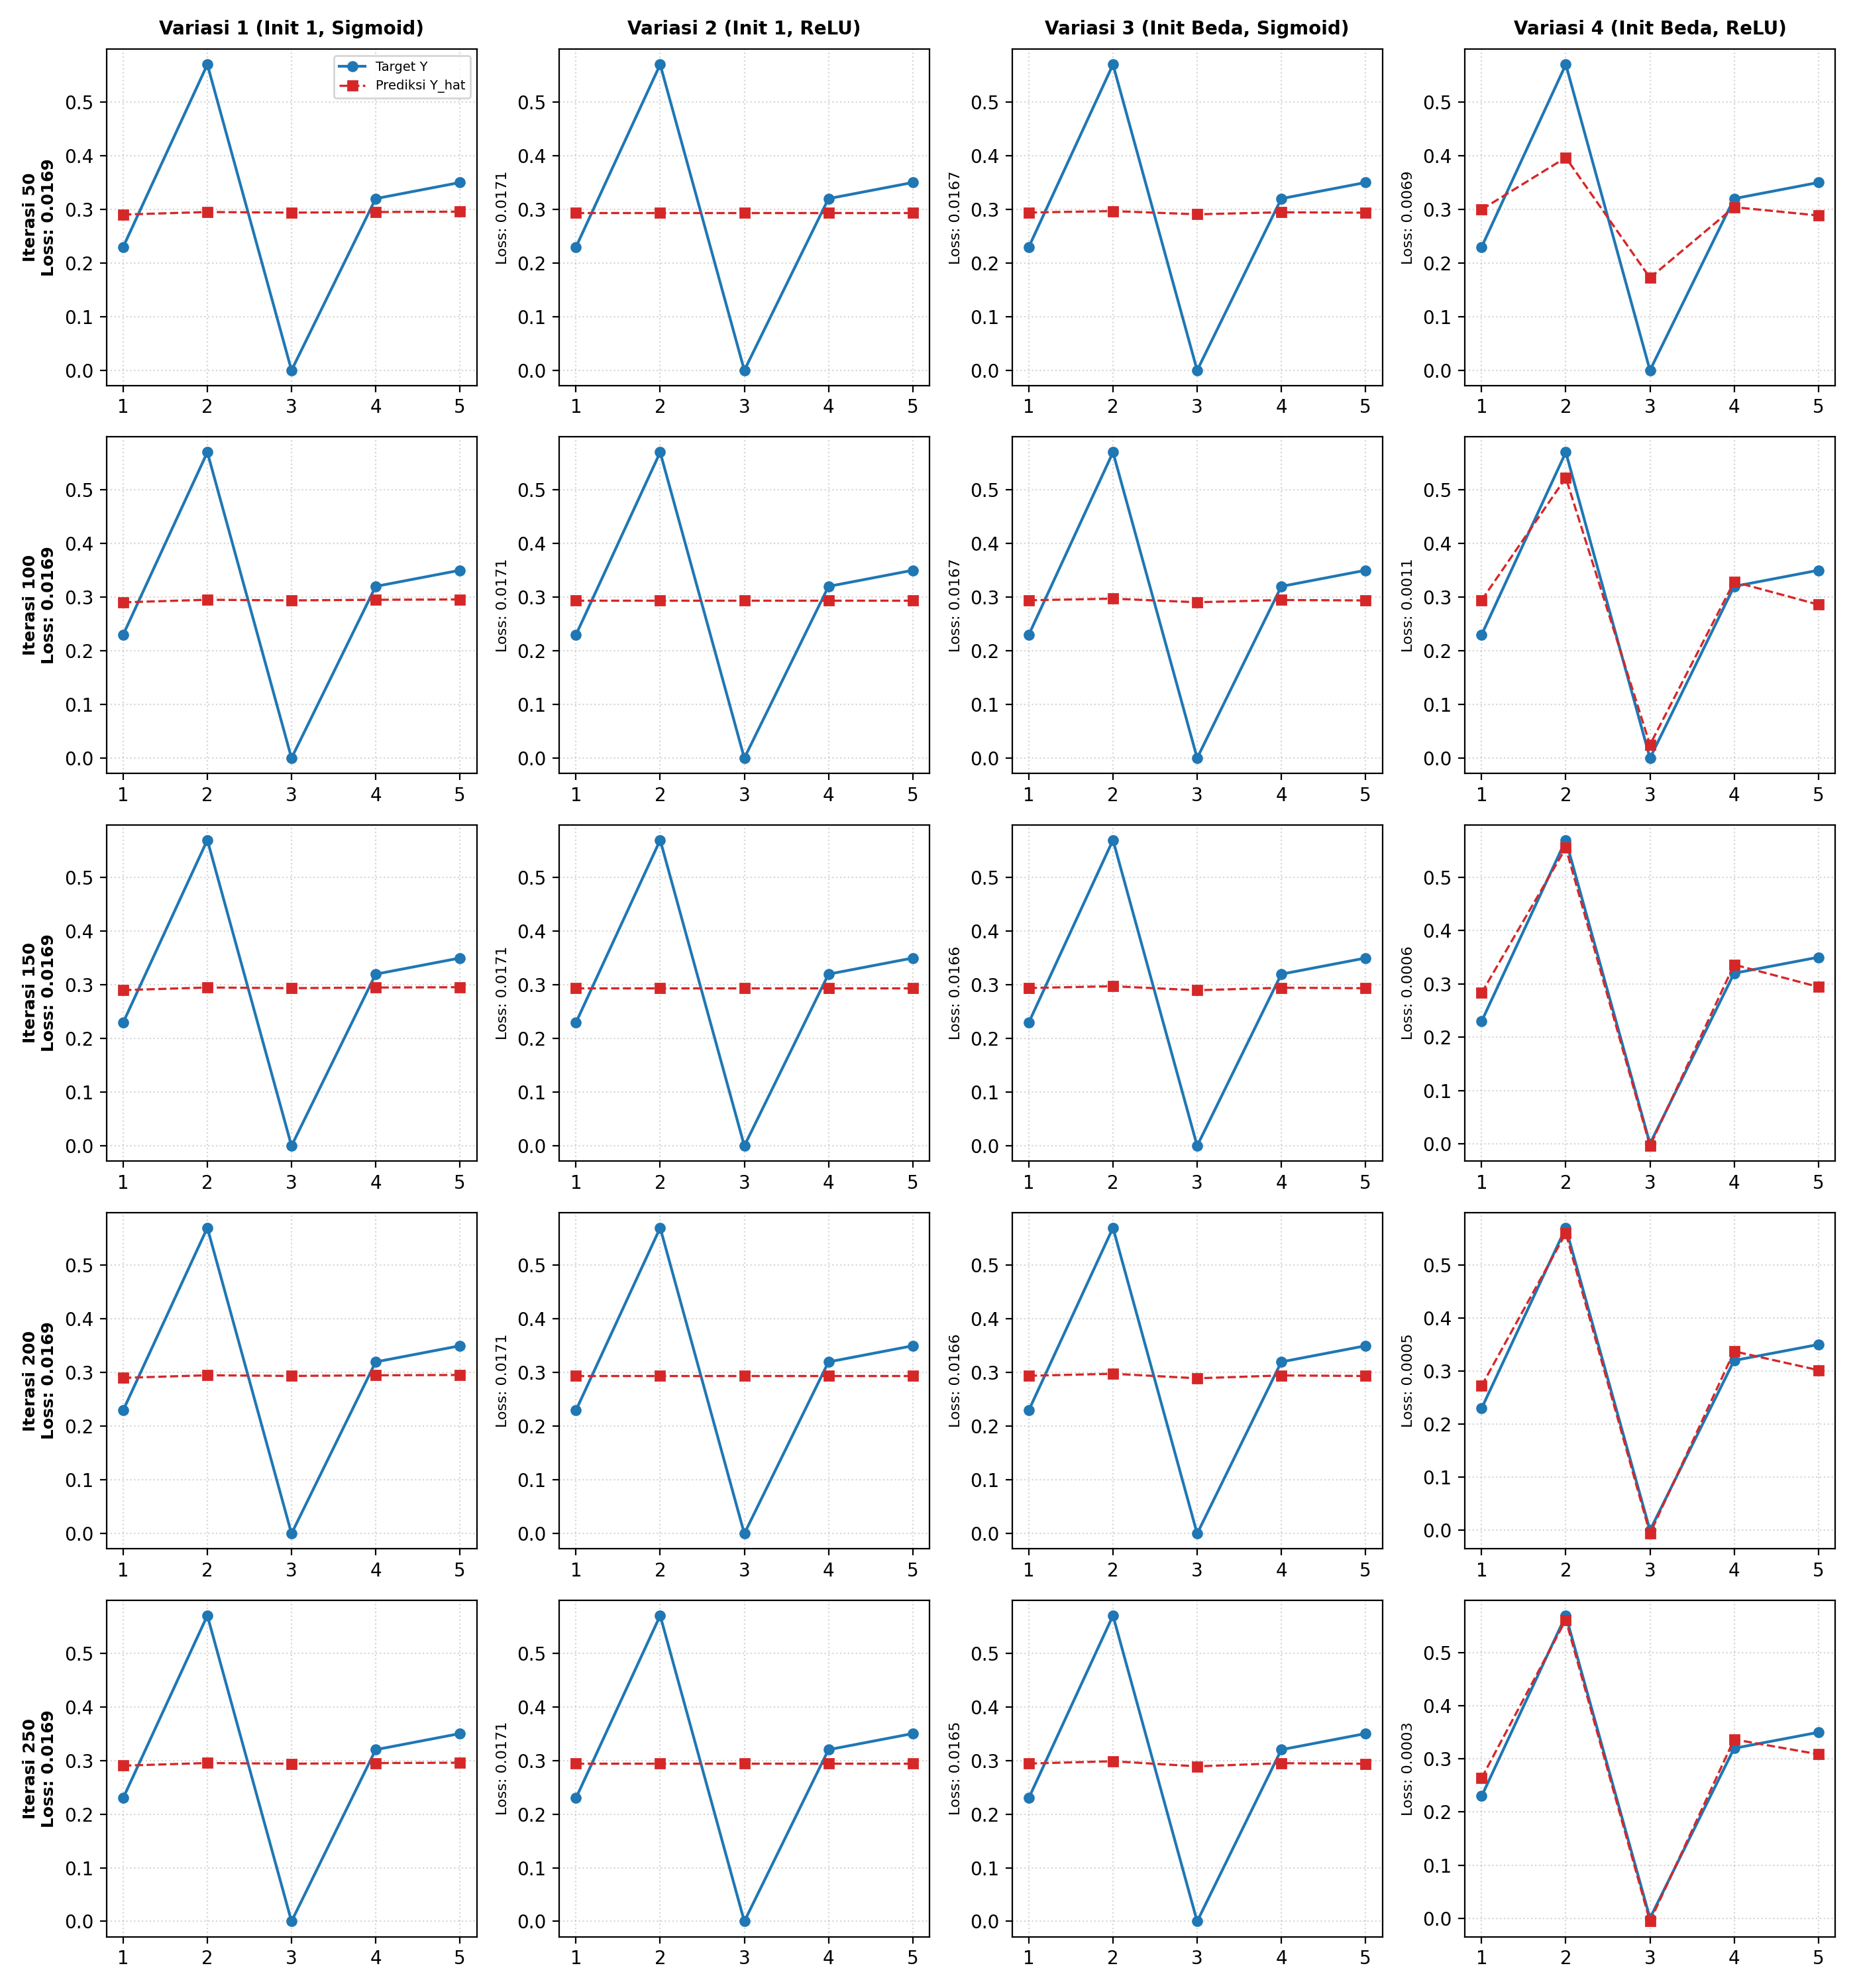
\includegraphics[width=0.98\textwidth]{grid_skalar_r3_r1_part1.png}
    \caption{Visualisasi Komparasi Target vs Prediksi Bobot Skalar $\mathbb{R}^3 \to \mathbb{R}^1$ (Bagian 1: Iterasi 50 s.d. 250).}
    \label{fig:grid_skalar_r1_p1}
\end{figure}

\clearpage
\begin{figure}[H]
    \centering
    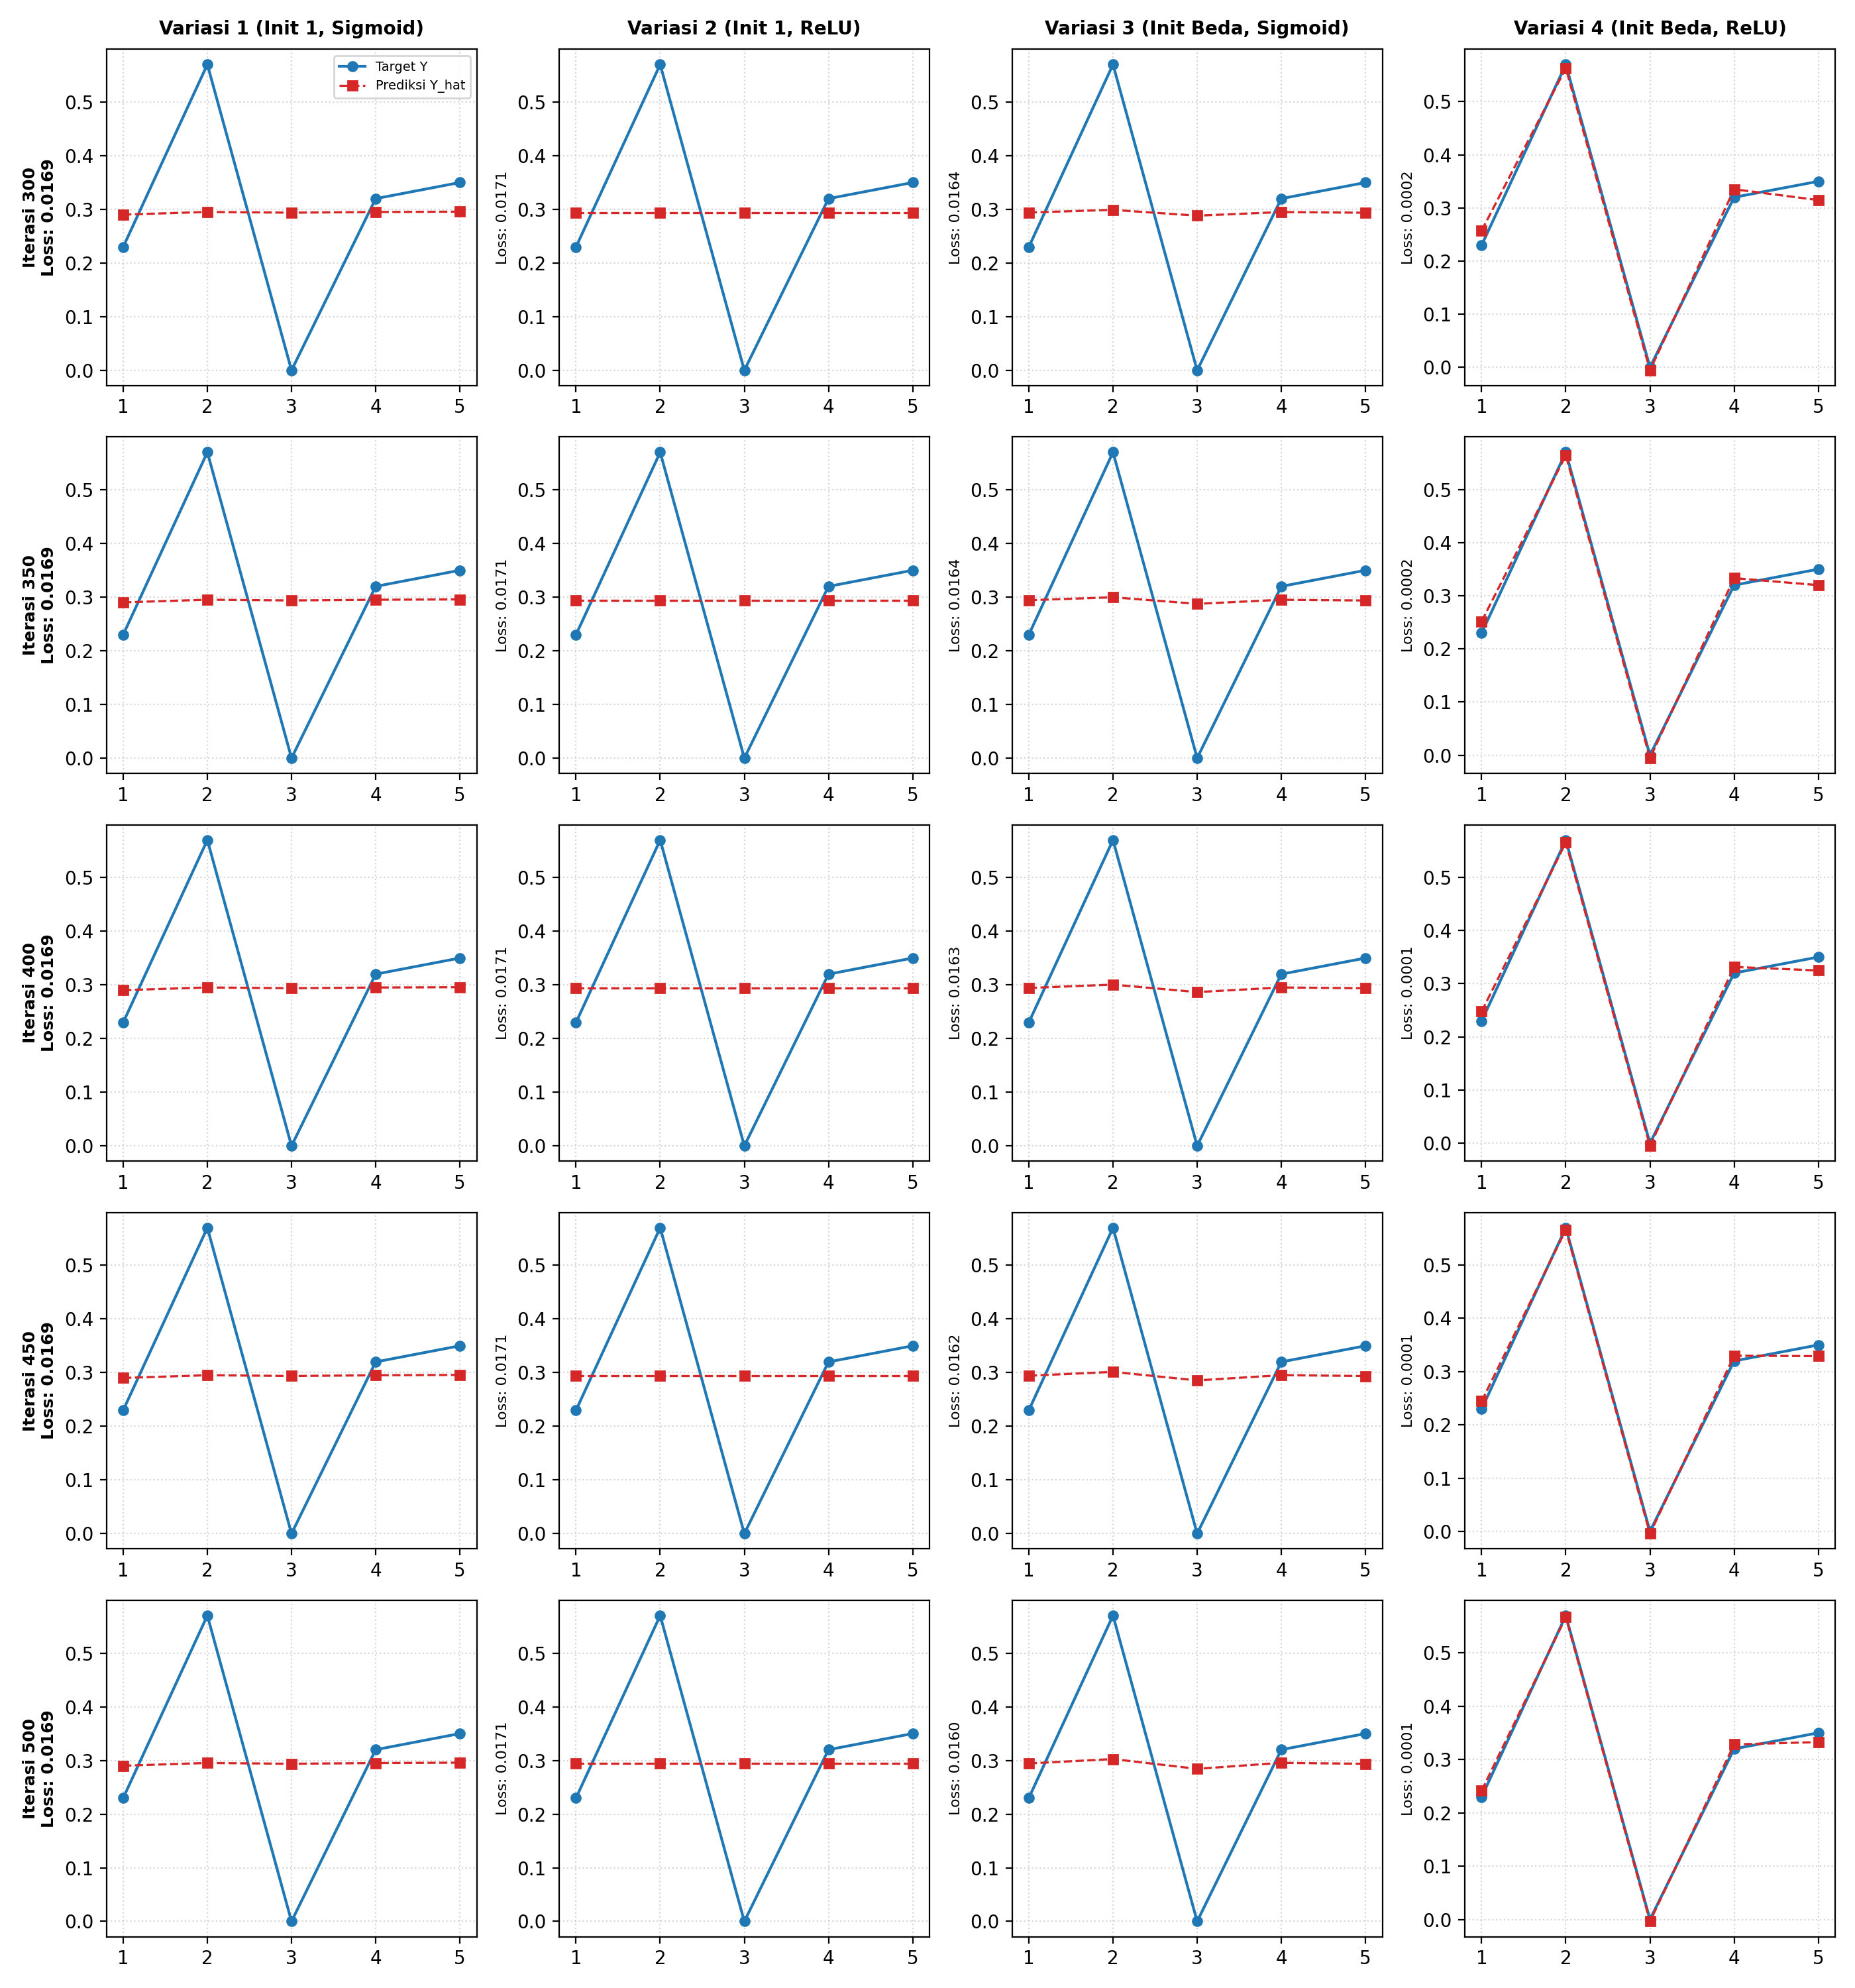
\includegraphics[width=0.98\textwidth]{grid_skalar_r3_r1_part2.png}
    \caption{Visualisasi Komparasi Target vs Prediksi Bobot Skalar $\mathbb{R}^3 \to \mathbb{R}^1$ (Bagian 2: Iterasi 300 s.d. 500).}
    \label{fig:grid_skalar_r1_p2}
\end{figure}

\clearpage
\subsubsection{Visualisasi Kurva Fungsi Loss: Bobot Skalar \texorpdfstring{$\mathbb{R}^3 \to \mathbb{R}^1$}{R3 -> R1}}
\label{subsubsec:loss_skalar_r1}

\begin{figure}[H]
    \centering
    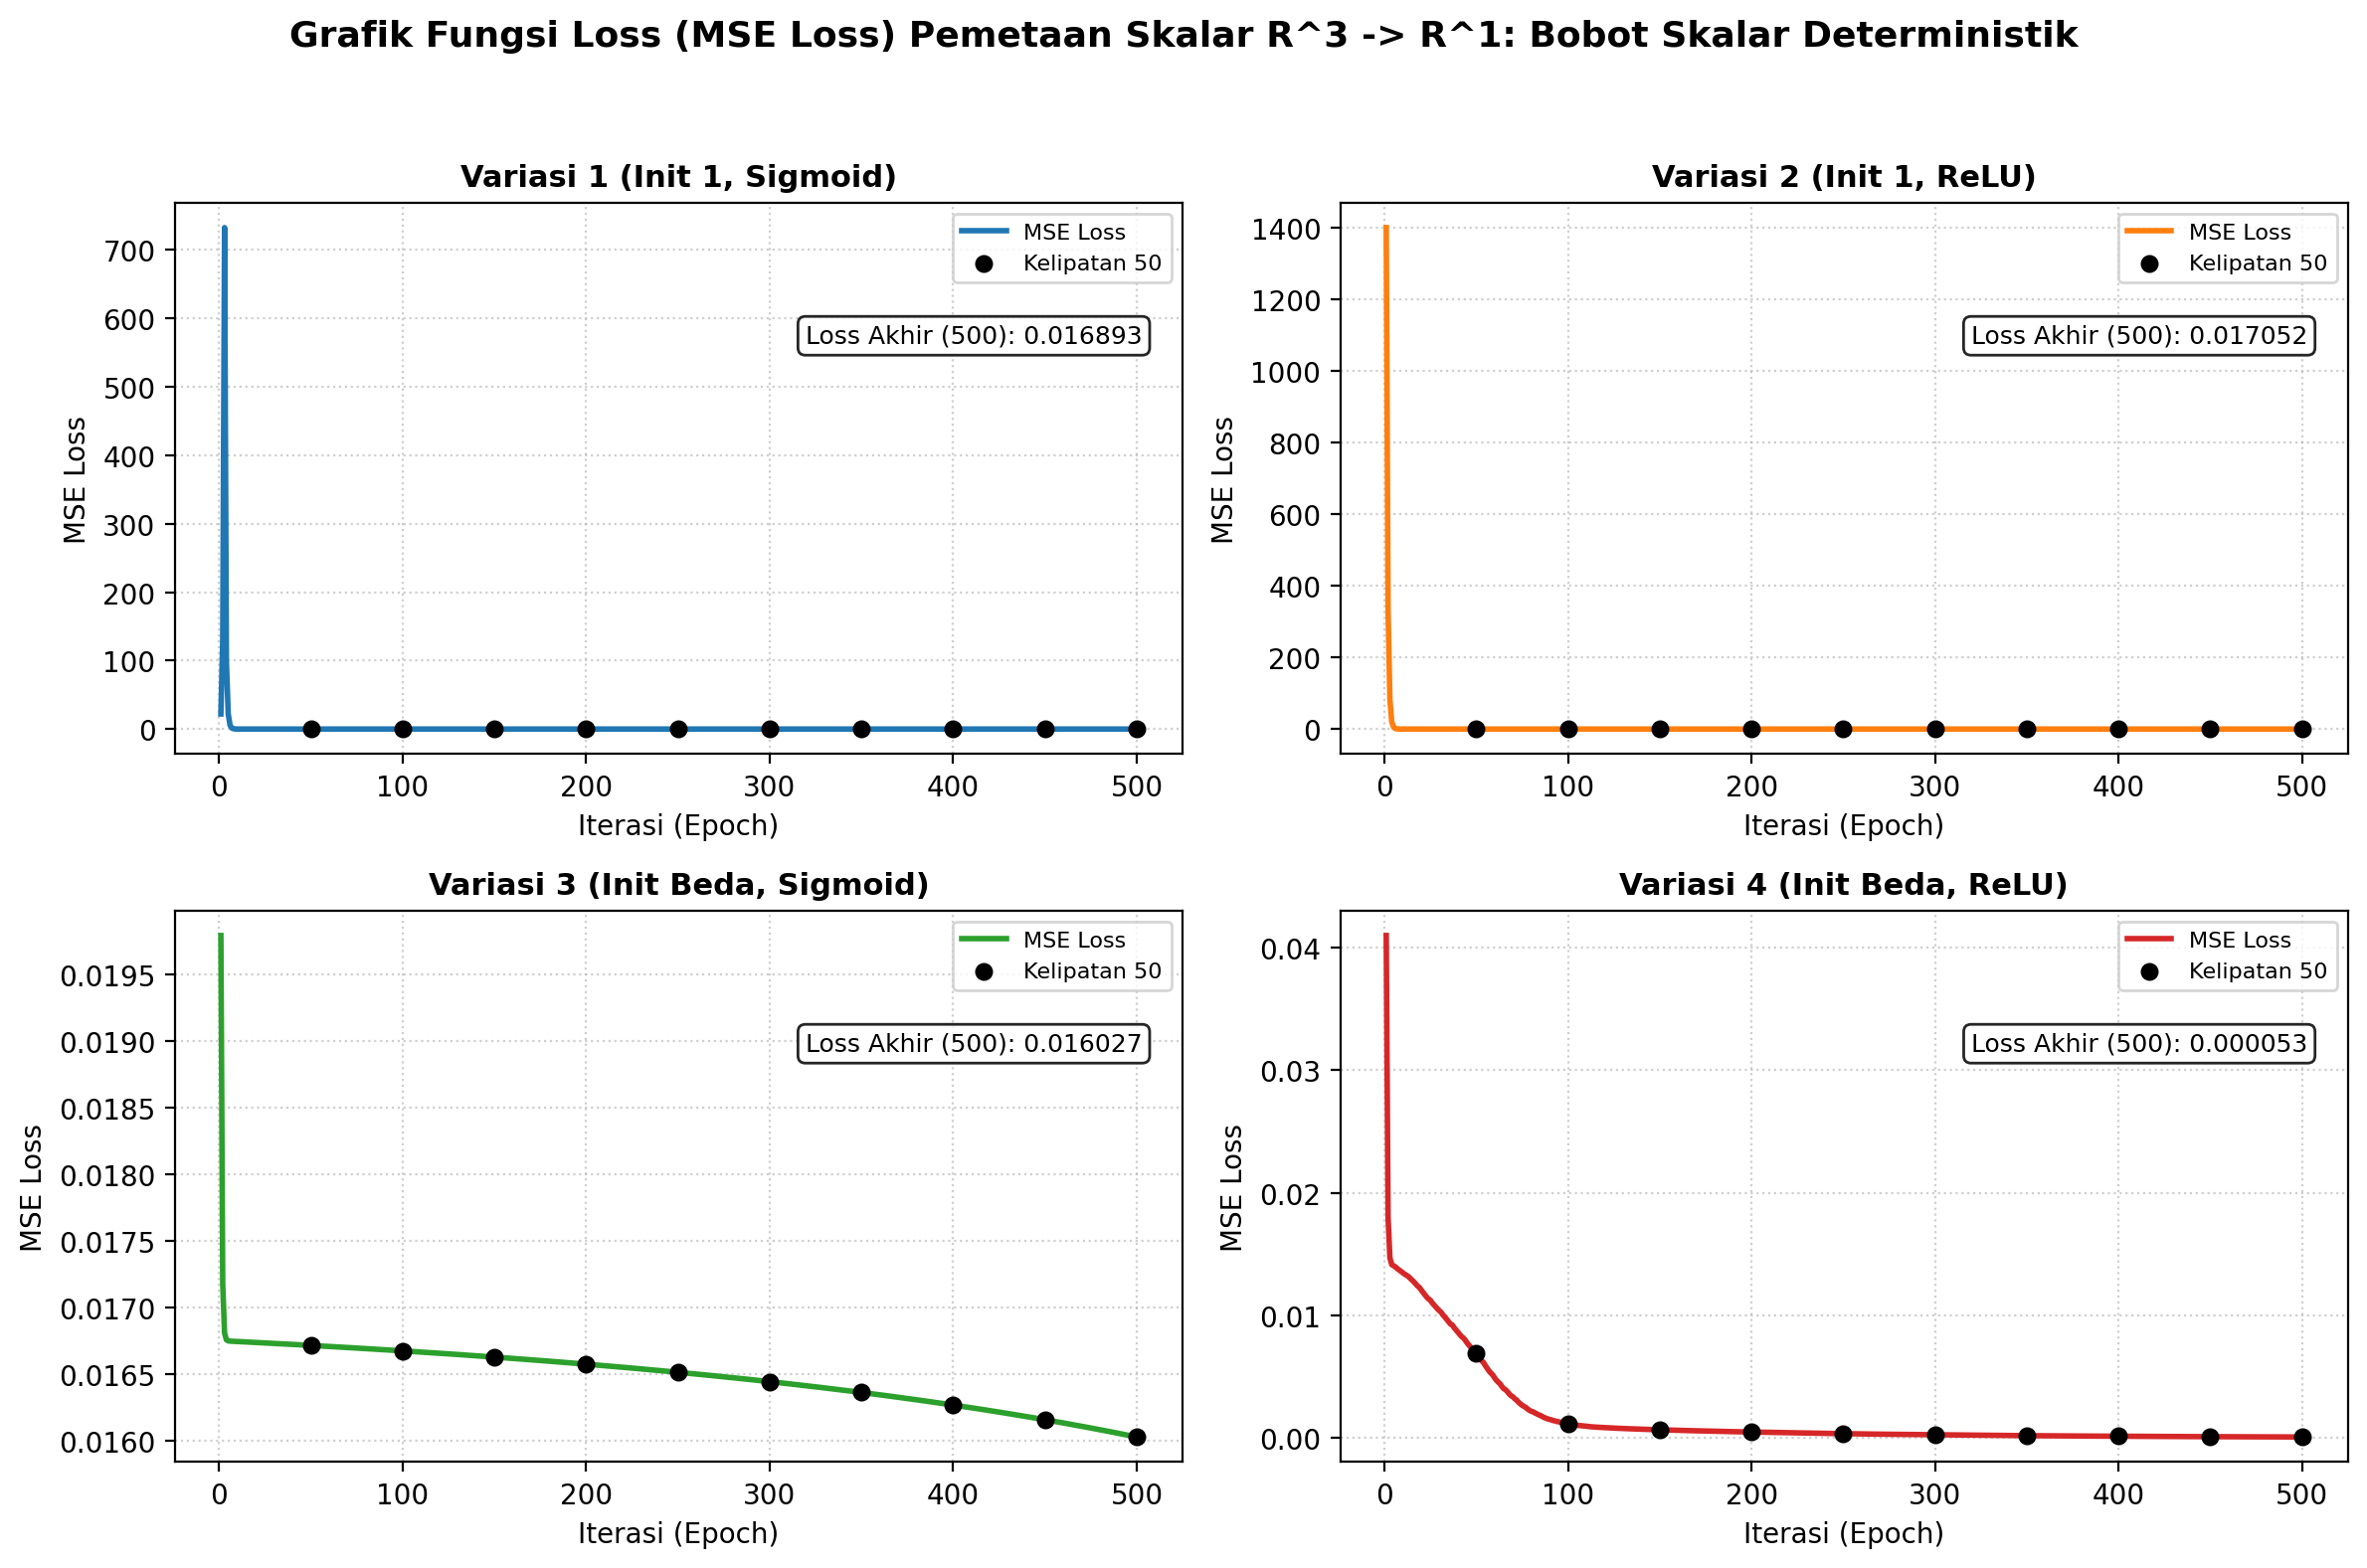
\includegraphics[width=0.98\textwidth]{loss_skalar_r3_r1.png}
    \caption{Grafik Fungsi Loss (MSE Loss) Pemetaan Skalar $\mathbb{R}^3 \to \mathbb{R}^1$ Bobot Skalar Deterministik pada 4 Variasi (Iterasi 1 s.d. 500).}
    \label{fig:loss_skalar_r1}
\end{figure}

% -------------------------------------------------------------------------
\clearpage
\subsection{Subkasus 2: Pemetaan Multi-Output \texorpdfstring{$\mathbb{R}^3 \to \mathbb{R}^2$}{R3 -> R2}}
\label{subsec:skalar_r3_r2}

\noindent Pada pemetaan multi-output ($n_3 = 2$), matriks parameter output layer berdimensi $W^{(3)} \in \mathbb{R}^{6 \times 2}$ dan $\mathbf{b}^{(3)} \in \mathbb{R}^{1 \times 2}$. Matriks prediksi berukuran $\hat{Y} \in \mathbb{R}^{5 \times 2}$.

\subsubsection{Tabel Komparasi 4 Variasi: Bobot Skalar \texorpdfstring{$\mathbb{R}^3 \to \mathbb{R}^2$}{R3 -> R2}}
\label{subsubsec:tabel_skalar_r2}

\begin{table}[H]
    \centering
    \small
    \caption{Perbandingan Nilai MSE Loss ($\mathcal{L}$) Setiap Kelipatan 50 Iterasi pada Pemetaan Multi-Output $\mathbb{R}^3 \to \mathbb{R}^2$ (Bobot Skalar Deterministik).}
    \label{tab:komparasi_skalar_r2}
    \begin{tabularx}{\textwidth}{c *{4}{>{\centering\arraybackslash}X}}
        \toprule
        \textbf{Iterasi} & \textbf{Variasi 1} & \textbf{Variasi 2} & \textbf{Variasi 3} & \textbf{Variasi 4} \\
        \textbf{($n$)} & \textbf{(Init 1, Sig)} & \textbf{(Init 1, ReLU)} & \textbf{(Init Beda, Sig)} & \textbf{(Init Beda, ReLU)} \\
        \midrule
        1    & 44.969629 & 2810.066210 & 0.033234 & 0.064531 \\
        2    & 264.181606 & 658.179571 & 0.025726 & 0.028872 \\
        50   & 0.025144 & 0.025144 & 0.024568 & 0.005405 \\
        100  & 0.025144 & 0.025144 & 0.024471 & 0.001851 \\
        150  & 0.025144 & 0.025144 & 0.024357 & 0.001604 \\
        200  & 0.025144 & 0.025144 & 0.024221 & 0.001488 \\
        250  & 0.025144 & 0.025144 & 0.024057 & 0.001394 \\
        300  & 0.025144 & 0.025144 & 0.023859 & 0.001309 \\
        350  & 0.025144 & 0.025144 & 0.023616 & 0.001225 \\
        400  & 0.025144 & 0.025144 & 0.023317 & 0.001148 \\
        450  & 0.025144 & 0.025144 & 0.022944 & 0.001064 \\
        500  & 0.025144 & 0.025144 & 0.022477 & 0.000980 \\
        \bottomrule
    \end{tabularx}
\end{table}

\subsubsection{Visualisasi Kurva Fungsi Loss: Bobot Skalar \texorpdfstring{$\mathbb{R}^3 \to \mathbb{R}^2$}{R3 -> R2}}
\label{subsubsec:loss_skalar_r2}

\begin{figure}[H]
    \centering
    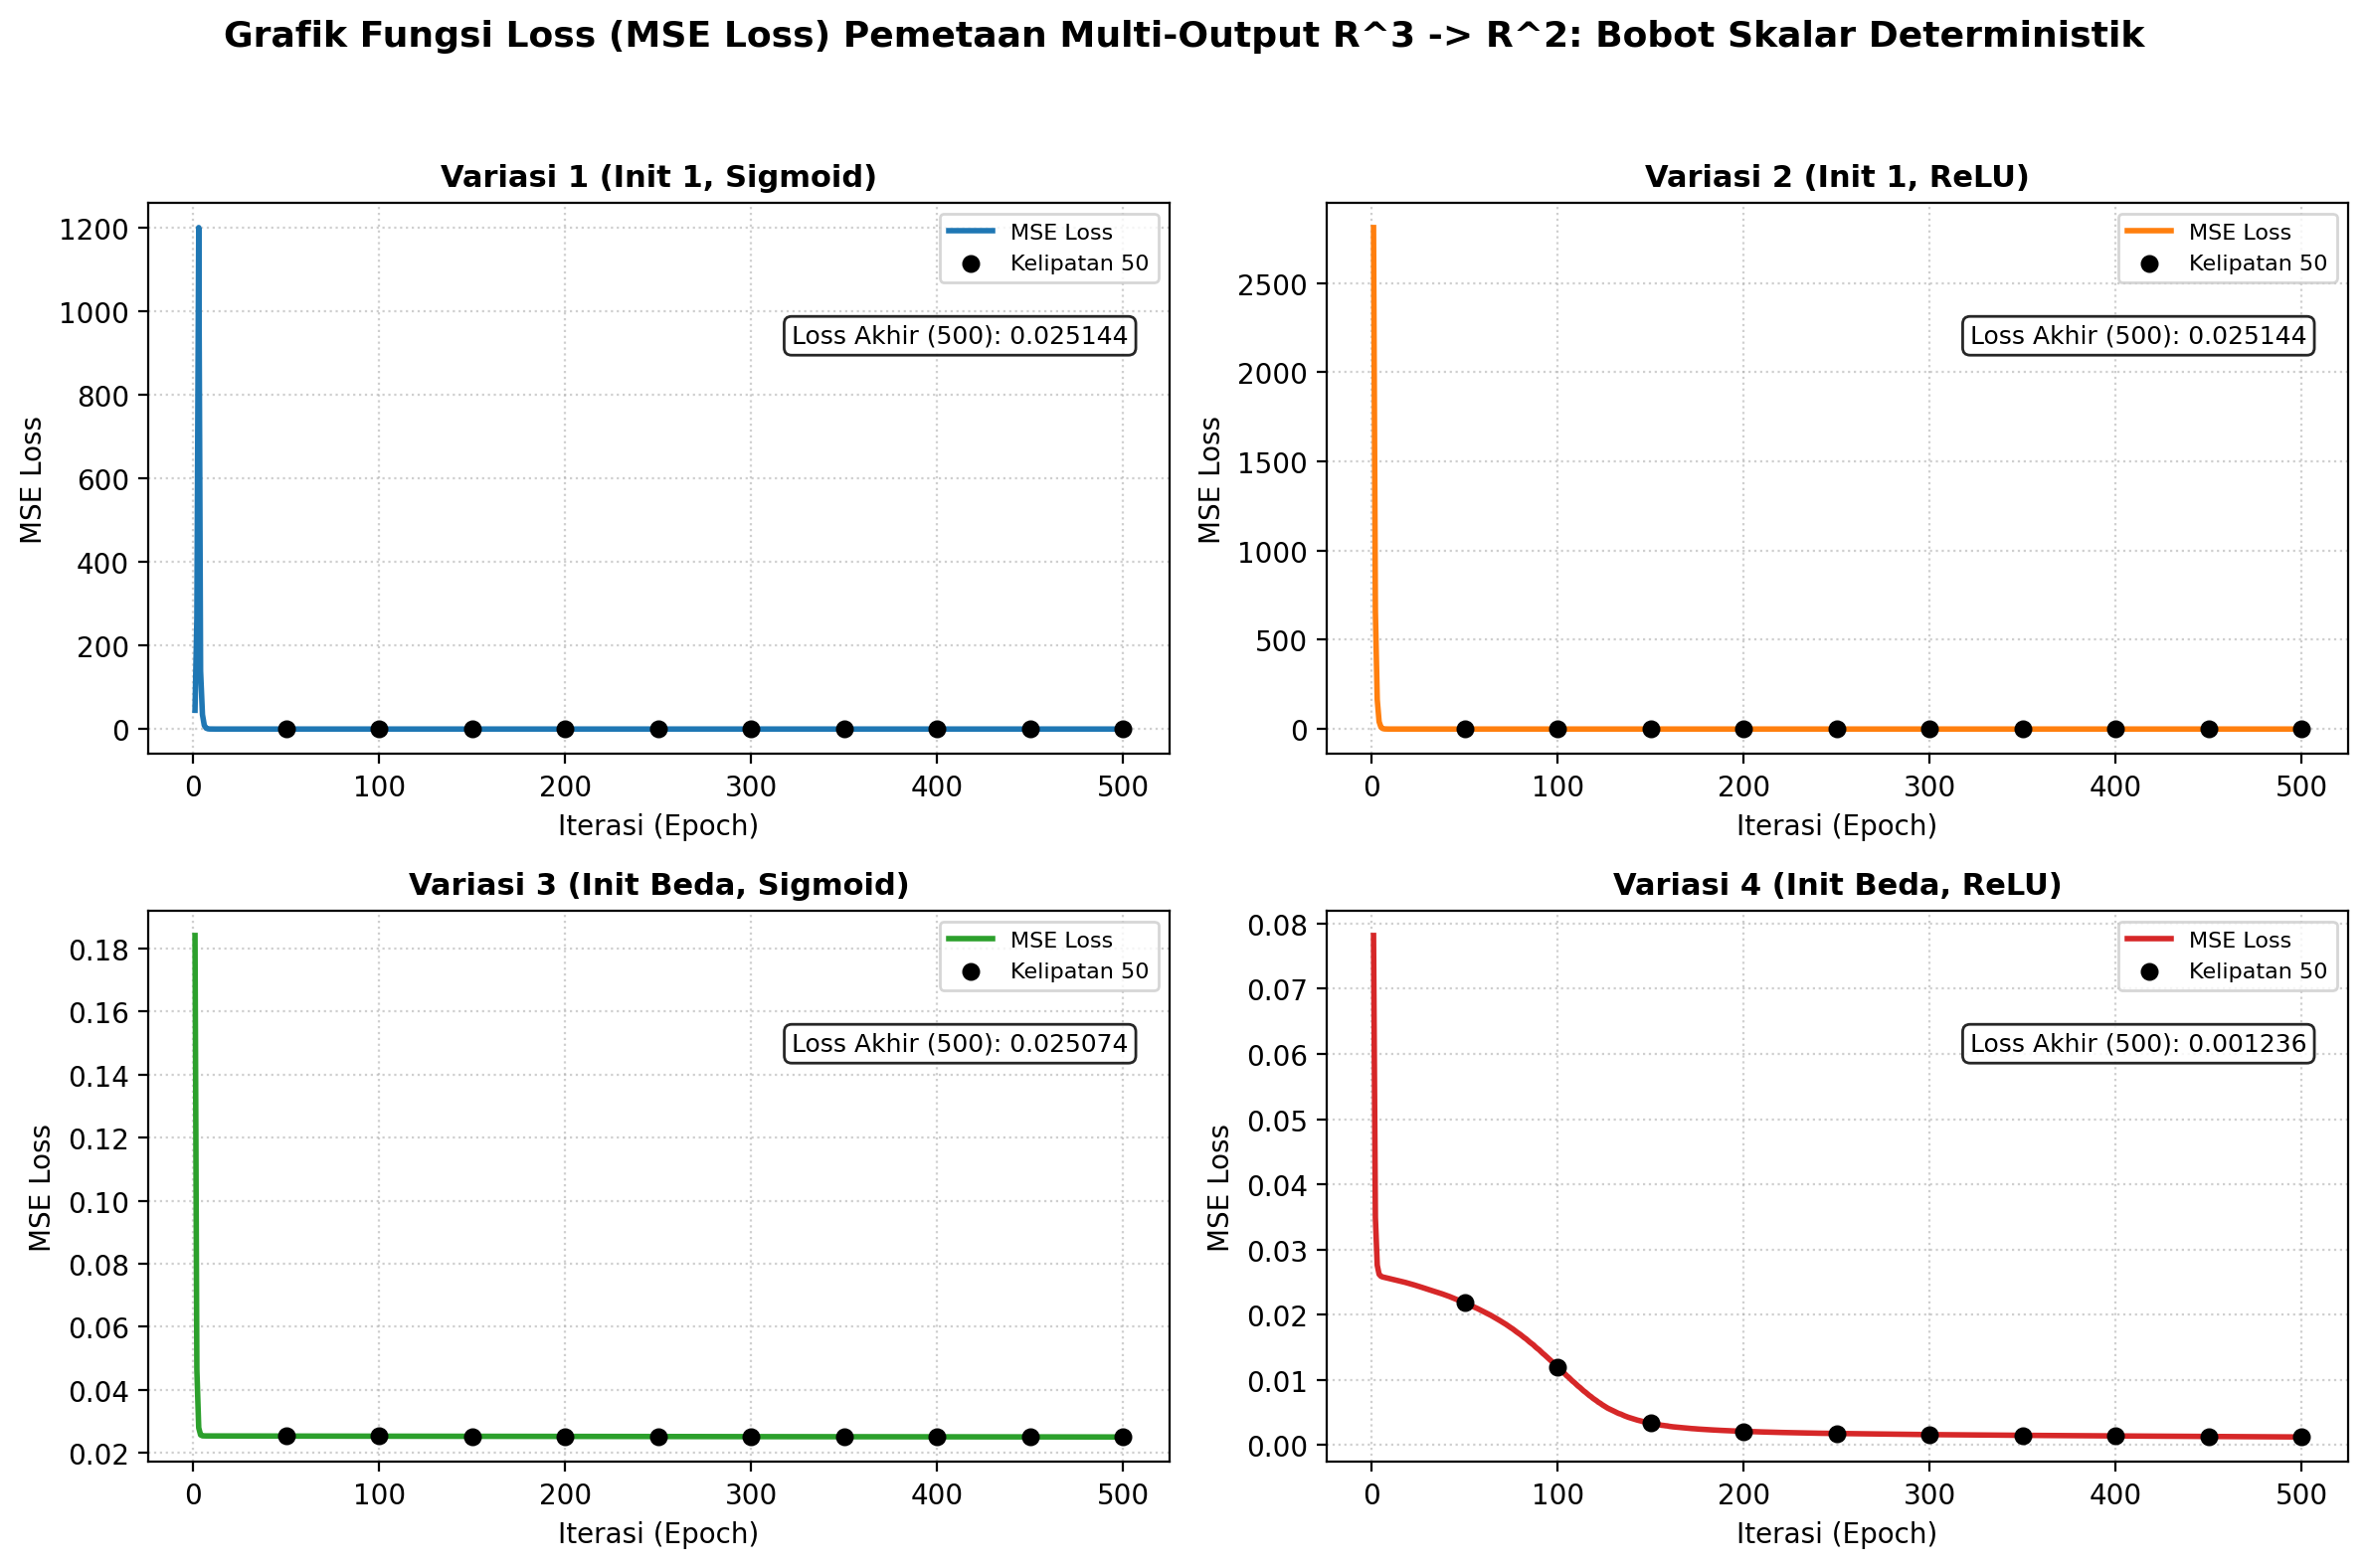
\includegraphics[width=0.98\textwidth]{loss_skalar_r3_r2.png}
    \caption{Grafik Fungsi Loss (MSE Loss) Pemetaan Multi-Output $\mathbb{R}^3 \to \mathbb{R}^2$ Bobot Skalar Deterministik pada 4 Variasi (Iterasi 1 s.d. 500).}
    \label{fig:loss_skalar_r2}
\end{figure}

% =========================================================================
% 3. KASUS 2: BOBOT BERDISTRIBUSI (REPARAMETERIZATION TRICK)
% =========================================================================
\clearpage
\section{Kasus 2: Bobot Berdistribusi (Reparameterization Trick)}
\label{sec:bobot_distribusi}

\subsection{Formulasi Reparameterization Trick}
\label{subsec:reparam_formula}

\noindent Matriks bobot pada layer $\ell$ dimodelkan sebagai variabel acak Gaussian yang direparameterisasi melalui matriks nilai rata-rata $M^{(\ell)}$, matriks simpangan baku $\Sigma^{(\ell)}$, dan matriks variabel acak normal baku $Z^{(\ell)} \sim \mathcal{N}(0, I)$:
\begin{equation}
    W^{(\ell)} = M^{(\ell)} + \Sigma^{(\ell)} \odot Z^{(\ell)} \in \mathbb{R}^{n_{\ell-1} \times n_\ell} \label{eq:reparam_matrix}
\end{equation}
Gradien terhadap parameter distribusi pada layer $\ell$ dihitung dari $\frac{\partial \mathcal{L}}{\partial H^{(\ell)}}$ (yang diturunkan secara rekursif dari layer $\ell+1$ melalui Persamaan \eqref{eq:chain_rule_h}):
\begin{equation}
    \frac{\partial \mathcal{L}}{\partial W^{(\ell)}} = \left(X^{(\ell-1)}\right)^T \frac{\partial \mathcal{L}}{\partial H^{(\ell)}}, \qquad
    \frac{\partial \mathcal{L}}{\partial M^{(\ell)}} = \frac{\partial \mathcal{L}}{\partial W^{(\ell)}}, \qquad
    \frac{\partial \mathcal{L}}{\partial \Sigma^{(\ell)}} = \frac{\partial \mathcal{L}}{\partial W^{(\ell)}} \odot Z^{(\ell)} \label{eq:reparam_gradients}
\end{equation}

% -------------------------------------------------------------------------
\subsection{Subkasus 1: Pemetaan Skalar \texorpdfstring{$\mathbb{R}^3 \to \mathbb{R}^1$}{R3 -> R1}}
\label{subsec:distribusi_r3_r1}

\subsubsection{Perhitungan Numerik 2 Iterasi (Variasi 1: Inisialisasi 1 Semua, Sigmoid, Seed 67)}
\label{subsubsec:distribusi_r1_hitung2iterasi}

\noindent Inisialisasi parameter awal ($M = \mathbf{1}, \Sigma = \mathbf{1}, \mathbf{b} = \mathbf{1}$):
\begin{equation}
    M^{(1)}_1 = \Sigma^{(1)}_1 = \mathbf{1}_{3 \times 4}, \; \mathbf{b}^{(1)}_1 = \mathbf{1}_{1 \times 4}, \; M^{(2)}_1 = \Sigma^{(2)}_1 = \mathbf{1}_{4 \times 6}, \; \mathbf{b}^{(2)}_1 = \mathbf{1}_{1 \times 6}, \; M^{(3)}_1 = \Sigma^{(3)}_1 = \mathbf{1}_{6 \times 1}, \; \mathbf{b}^{(3)}_1 = [1.0]
\end{equation}

\noindent \textbf{Iterasi ke-1}:
\begin{enumerate}
    \item \textit{Pengambilan Sampel Variabel Acak Normal Baku ($Z^{(\ell)}_1 \sim \mathcal{N}(0, I)$, seed 67) \& Konstruksi Bobot}:
    \begin{align}
        Z^{(1)}_1 &= \begin{bmatrix}
             1.1285 &  0.1442 & -1.1153 &  1.2310 \\
            -0.1547 & -0.5984 &  0.3490 &  1.2206 \\
            -0.8287 & -1.1111 & -0.5243 & -1.0934
        \end{bmatrix} \\[0.2em]
        W^{(1)}_1 &= M^{(1)}_1 + \Sigma^{(1)}_1 \odot Z^{(1)}_1 = \begin{bmatrix}
            2.1285 &  1.1442 & -0.1153 &  2.2310 \\
            0.8453 &  0.4016 &  1.3490 &  2.2206 \\
            0.1713 & -0.1111 &  0.4757 & -0.0934
        \end{bmatrix} \\[0.2em]
        Z^{(2)}_1 &= \begin{bmatrix}
            -1.6353 & -1.6850 &  0.6923 & -2.3886 & -0.7544 & -1.0532 \\
             1.7835 &  0.4447 &  0.1186 &  0.5277 & -1.6998 & -1.1453 \\
            -0.5844 &  0.9073 &  0.5345 &  0.0515 &  0.5821 & -0.8083 \\
            -0.0859 &  0.3117 & -1.0321 &  0.9448 & -0.8261 & -1.0630
        \end{bmatrix} \\[0.2em]
        W^{(2)}_1 &= M^{(2)}_1 + \Sigma^{(2)}_1 \odot Z^{(2)}_1 = \begin{bmatrix}
            -0.6353 & -0.6850 &  1.6923 & -1.3886 &  0.2456 & -0.0532 \\
             2.7835 &  1.4447 &  1.1186 &  1.5277 & -0.6998 & -0.1453 \\
             0.4156 &  1.9073 &  1.5345 &  1.0515 &  1.5821 &  0.1917 \\
             0.9141 &  1.3117 & -0.0321 &  1.9448 &  0.1739 & -0.0630
        \end{bmatrix} \\[0.2em]
        Z^{(3)}_1 &= \begin{bmatrix} 0.6063 & -0.2070 & -0.7565 & -2.3861 & 0.8739 & -0.1124 \end{bmatrix}^T \\[0.2em]
        W^{(3)}_1 &= M^{(3)}_1 + \Sigma^{(3)}_1 \odot Z^{(3)}_1 = \begin{bmatrix} 1.6063 & 0.7930 & 0.2435 & -1.3861 & 1.8739 & 0.8876 \end{bmatrix}^T
    \end{align}

    \item \textit{Forward Pass}:
    \begin{align}
        H^{(1)}_1 &= X W^{(1)}_1 + \mathbf{1}_5 \mathbf{b}^{(1)}_1 = \begin{bmatrix}
            1.4333 & 1.1614 & 1.4010 & 1.6392 \\
            2.0216 & 1.4423 & 1.3267 & 2.0678 \\
            1.9500 & 1.4587 & 1.8339 & 2.7692 \\
            2.3521 & 1.6704 & 1.4422 & 2.7630 \\
            2.0452 & 1.4595 & 1.6953 & 2.5202
        \end{bmatrix} \\[0.2em]
        X^{(1)}_1 &= \sigma\!\left(H^{(1)}_1\right) = \begin{bmatrix}
            0.8074 & 0.7616 & 0.8023 & 0.8374 \\
            0.8830 & 0.8088 & 0.7903 & 0.8877 \\
            0.8755 & 0.8113 & 0.8622 & 0.9410 \\
            0.9131 & 0.8416 & 0.8088 & 0.9406 \\
            0.8855 & 0.8115 & 0.8449 & 0.9255
        \end{bmatrix} \\[0.2em]
        H^{(2)}_1 &= X^{(1)}_1 W^{(2)}_1 + \mathbf{1}_5 \mathbf{b}^{(2)}_1 = \begin{bmatrix}
            3.7058 & 4.1759 & 4.4227 & 3.5146 & 2.0804 & 0.9474 \\
            3.8302 & 4.2353 & 4.5834 & 3.5669 & 2.0556 & 0.9311 \\
            3.9206 & 4.4512 & 4.6820 & 3.7605 & 2.1750 & 0.9416 \\
            3.9585 & 4.3668 & 4.6977 & 3.6976 & 2.0785 & 0.9249 \\
            3.8933 & 4.3912 & 4.6730 & 3.6985 & 2.1473 & 0.9387
        \end{bmatrix} \\[0.2em]
        X^{(2)}_1 &= \sigma\!\left(H^{(2)}_1\right) = \begin{bmatrix}
            0.9760 & 0.9849 & 0.9881 & 0.9711 & 0.8890 & 0.7206 \\
            0.9788 & 0.9857 & 0.9899 & 0.9725 & 0.8865 & 0.7173 \\
            0.9806 & 0.9885 & 0.9908 & 0.9773 & 0.8980 & 0.7194 \\
            0.9813 & 0.9875 & 0.9910 & 0.9758 & 0.8888 & 0.7160 \\
            0.9800 & 0.9878 & 0.9907 & 0.9758 & 0.8954 & 0.7188
        \end{bmatrix} \\[0.2em]
        \hat{Y}_1 &= H^{(3)}_1 = X^{(2)}_1 W^{(3)}_1 + \mathbf{1}_5 \mathbf{b}^{(3)}_1 = \begin{bmatrix} 4.5488 & 4.5448 & 4.5669 & 4.5491 & 4.5621 \end{bmatrix}^T \\[0.2em]
        \mathcal{L}_1 &= \frac{1}{2N} \sum_{i=1}^5 \left( y_i - \hat{y}_{i, 1} \right)^2 = 9.093420
    \end{align}

    \item \textit{Backward Pass}:
    \begin{itemize}
        \item \textbf{Layer 3 ($\ell = 3$)}:
        \begin{align}
            \frac{\partial \mathcal{L}}{\partial H^{(3)}_1} &= \frac{1}{5}\left(\hat{Y}_1 - Y\right) = \begin{bmatrix} 0.8638 & 0.7950 & 0.9134 & 0.8458 & 0.8424 \end{bmatrix}^T \\[0.2em]
            \frac{\partial \mathcal{L}}{\partial M^{(3)}_1} &= \left(X^{(2)}_1\right)^T \frac{\partial \mathcal{L}}{\partial H^{(3)}_1} = \begin{bmatrix} 4.1723 & 4.2045 & 4.2182 & 4.1519 & 3.7989 & 3.0609 \end{bmatrix}^T \\[0.2em]
            \frac{\partial \mathcal{L}}{\partial \Sigma^{(3)}_1} &= \frac{\partial \mathcal{L}}{\partial M^{(3)}_1} \odot Z^{(3)}_1 = \begin{bmatrix} 2.5297 & -0.8703 & -3.1910 & -9.9070 & 3.3199 & -0.3442 \end{bmatrix}^T \\[0.2em]
            \frac{\partial \mathcal{L}}{\partial \mathbf{b}^{(3)}_1} &= \mathbf{1}_5^T \frac{\partial \mathcal{L}}{\partial H^{(3)}_1} = [4.2603]
        \end{align}
        \item \textbf{Layer 2 ($\ell = 2$, membutuhkan $\frac{\partial \mathcal{L}}{\partial H^{(3)}_1}$ dan $W^{(3)}_1$ dari layer $\ell+1 = 3$)}:
        \begin{align}
            \frac{\partial \mathcal{L}}{\partial X^{(2)}_1} &= \frac{\partial \mathcal{L}}{\partial H^{(3)}_1} \left(W^{(3)}_1\right)^T = \begin{bmatrix}
                1.3875 & 0.6850 & 0.2103 & -1.1973 & 1.6186 & 0.7666 \\
                1.2769 & 0.6304 & 0.1936 & -1.1019 & 1.4897 & 0.7056 \\
                1.4672 & 0.7243 & 0.2224 & -1.2660 & 1.7116 & 0.8107 \\
                1.3586 & 0.6707 & 0.2060 & -1.1724 & 1.5850 & 0.7507 \\
                1.3532 & 0.6680 & 0.2051 & -1.1677 & 1.5786 & 0.7477
            \end{bmatrix} \\[0.2em]
            \frac{\partial \mathcal{L}}{\partial H^{(2)}_1} &= \frac{\partial \mathcal{L}}{\partial X^{(2)}_1} \odot \sigma'\!\left(H^{(2)}_1\right) = \begin{bmatrix}
                0.0325 & 0.0102 & 0.0025 & -0.0336 & 0.1597 & 0.1543 \\
                0.0266 & 0.0089 & 0.0019 & -0.0294 & 0.1499 & 0.1431 \\
                0.0280 & 0.0083 & 0.0020 & -0.0281 & 0.1568 & 0.1636 \\
                0.0250 & 0.0083 & 0.0018 & -0.0277 & 0.1567 & 0.1526 \\
                0.0265 & 0.0081 & 0.0019 & -0.0275 & 0.1478 & 0.1511
            \end{bmatrix} \\[0.2em]
            \frac{\partial \mathcal{L}}{\partial M^{(2)}_1} &= \left(X^{(1)}_1\right)^T \frac{\partial \mathcal{L}}{\partial H^{(2)}_1} = \begin{bmatrix}
                0.1204 & 0.0380 & 0.0088 & -0.1274 & 0.6725 & 0.6674 \\
                0.1114 & 0.0352 & 0.0082 & -0.1179 & 0.6219 & 0.6171 \\
                0.1137 & 0.0358 & 0.0083 & -0.1201 & 0.6334 & 0.6291 \\
                0.1251 & 0.0395 & 0.0092 & -0.1323 & 0.6985 & 0.6937
            \end{bmatrix} \\[0.2em]
            \frac{\partial \mathcal{L}}{\partial \Sigma^{(2)}_1} &= \frac{\partial \mathcal{L}}{\partial M^{(2)}_1} \odot Z^{(2)}_1 = \begin{bmatrix}
                -0.1969 & -0.0641 &  0.0061 &  0.3043 & -0.5074 & -0.7029 \\
                 0.1987 &  0.0156 &  0.0010 & -0.0622 & -1.0571 & -0.7068 \\
                -0.0665 &  0.0325 &  0.0045 & -0.0062 &  0.3687 & -0.5086 \\
                -0.0107 &  0.0123 & -0.0095 & -0.1249 & -0.5771 & -0.7374
            \end{bmatrix} \\[0.2em]
            \frac{\partial \mathcal{L}}{\partial \mathbf{b}^{(2)}_1} &= \mathbf{1}_5^T \frac{\partial \mathcal{L}}{\partial H^{(2)}_1} = \begin{bmatrix} 0.1385 & 0.0437 & 0.0102 & -0.1464 & 0.7709 & 0.7648 \end{bmatrix}
        \end{align}
        \item \textbf{Layer 1 ($\ell = 1$, membutuhkan $\frac{\partial \mathcal{L}}{\partial H^{(2)}_1}$ dan $W^{(2)}_1$ dari layer $\ell+1 = 2$)}:
        \begin{align}
            \frac{\partial \mathcal{L}}{\partial X^{(1)}_1} &= \frac{\partial \mathcal{L}}{\partial H^{(2)}_1} \left(W^{(2)}_1\right)^T = \begin{bmatrix}
                0.0542 & -0.0776 & 0.2837 & -0.0043 \\
                0.0504 & -0.0818 & 0.2645 & -0.0044 \\
                0.0489 & -0.0844 & 0.2803 & -0.0014 \\
                0.0503 & -0.0905 & 0.2771 & -0.0025 \\
                0.0473 & -0.0800 & 0.2632 & -0.0026
            \end{bmatrix} \\[0.2em]
            \frac{\partial \mathcal{L}}{\partial H^{(1)}_1} &= \frac{\partial \mathcal{L}}{\partial X^{(1)}_1} \odot \sigma'\!\left(H^{(1)}_1\right) = \begin{bmatrix}
                0.0084 & -0.0141 & 0.0450 & -0.0006 \\
                0.0052 & -0.0126 & 0.0438 & -0.0004 \\
                0.0053 & -0.0129 & 0.0333 & -0.0001 \\
                0.0040 & -0.0121 & 0.0428 & -0.0001 \\
                0.0048 & -0.0122 & 0.0345 & -0.0002
            \end{bmatrix} \\[0.2em]
            \frac{\partial \mathcal{L}}{\partial M^{(1)}_1} &= X^T \frac{\partial \mathcal{L}}{\partial H^{(1)}_1} = \begin{bmatrix}
                0.0074 & -0.0188 & 0.0605 & -0.0004 \\
                0.0085 & -0.0204 & 0.0600 & -0.0003 \\
                0.0084 & -0.0191 & 0.0611 & -0.0005
            \end{bmatrix} \\[0.2em]
            \frac{\partial \mathcal{L}}{\partial \Sigma^{(1)}_1} &= \frac{\partial \mathcal{L}}{\partial M^{(1)}_1} \odot Z^{(1)}_1 = \begin{bmatrix}
                 0.0084 & -0.0027 & -0.0674 & -0.0005 \\
                -0.0013 &  0.0122 &  0.0209 & -0.0004 \\
                -0.0069 &  0.0213 & -0.0320 &  0.0005
            \end{bmatrix} \\[0.2em]
            \frac{\partial \mathcal{L}}{\partial \mathbf{b}^{(1)}_1} &= \mathbf{1}_5^T \frac{\partial \mathcal{L}}{\partial H^{(1)}_1} = \begin{bmatrix} 0.0278 & -0.0640 & 0.1995 & -0.0014 \end{bmatrix}
        \end{align}
    \end{itemize}

    \item \textit{Pembaruan Parameter ($\eta = 0.5$)}:
    \begin{align}
        M^{(3)}_2 &= M^{(3)}_1 - 0.5 \frac{\partial \mathcal{L}}{\partial M^{(3)}_1} = \begin{bmatrix} -1.0861 & -1.1022 & -1.1091 & -1.0760 & -0.8994 & -0.5305 \end{bmatrix}^T \\[0.2em]
        \Sigma^{(3)}_2 &= \Sigma^{(3)}_1 - 0.5 \frac{\partial \mathcal{L}}{\partial \Sigma^{(3)}_1} = \begin{bmatrix} -0.2648 & 1.4352 & 2.5955 & 5.9535 & -0.6599 & 1.1721 \end{bmatrix}^T \\[0.2em]
        \mathbf{b}^{(3)}_2 &= \mathbf{b}^{(3)}_1 - 0.5 \frac{\partial \mathcal{L}}{\partial \mathbf{b}^{(3)}_1} = [-1.1302] \\[0.2em]
        M^{(2)}_2 &= M^{(2)}_1 - 0.5 \frac{\partial \mathcal{L}}{\partial M^{(2)}_1} = \begin{bmatrix}
            0.9398 & 0.9810 & 0.9956 & 1.0637 & 0.6637 & 0.6663 \\
            0.9443 & 0.9824 & 0.9959 & 1.0589 & 0.6891 & 0.6914 \\
            0.9431 & 0.9821 & 0.9958 & 1.0601 & 0.6833 & 0.6854 \\
            0.9374 & 0.9803 & 0.9954 & 1.0661 & 0.6507 & 0.6532
        \end{bmatrix} \\[0.2em]
        \Sigma^{(2)}_2 &= \Sigma^{(2)}_1 - 0.5 \frac{\partial \mathcal{L}}{\partial \Sigma^{(2)}_1} = \begin{bmatrix}
            1.0985 & 1.0320 & 0.9969 & 0.8478 & 1.2537 & 1.3514 \\
            0.9006 & 0.9922 & 0.9995 & 1.0311 & 1.5285 & 1.3534 \\
            1.0332 & 0.9837 & 0.9978 & 1.0031 & 0.8156 & 1.2543 \\
            1.0054 & 0.9938 & 1.0047 & 1.0625 & 1.2885 & 1.3687
        \end{bmatrix} \\[0.2em]
        \mathbf{b}^{(2)}_2 &= \mathbf{b}^{(2)}_1 - 0.5 \frac{\partial \mathcal{L}}{\partial \mathbf{b}^{(2)}_1} = \begin{bmatrix} 0.9308 & 0.9781 & 0.9949 & 1.0732 & 0.6146 & 0.6176 \end{bmatrix} \\[0.2em]
        M^{(1)}_2 &= M^{(1)}_1 - 0.5 \frac{\partial \mathcal{L}}{\partial M^{(1)}_1} = \begin{bmatrix}
            0.9963 & 1.0094 & 0.9698 & 1.0002 \\
            0.9957 & 1.0102 & 0.9700 & 1.0002 \\
            0.9958 & 1.0096 & 0.9694 & 1.0003
        \end{bmatrix} \\[0.2em]
        \Sigma^{(1)}_2 &= \Sigma^{(1)}_1 - 0.5 \frac{\partial \mathcal{L}}{\partial \Sigma^{(1)}_1} = \begin{bmatrix}
            0.9958 & 1.0014 & 1.0337 & 1.0002 \\
            1.0007 & 0.9939 & 0.9895 & 1.0002 \\
            1.0035 & 0.9894 & 1.0160 & 0.9997
        \end{bmatrix} \\[0.2em]
        \mathbf{b}^{(1)}_2 &= \mathbf{b}^{(1)}_1 - 0.5 \frac{\partial \mathcal{L}}{\partial \mathbf{b}^{(1)}_1} = \begin{bmatrix} 0.9861 & 1.0320 & 0.9003 & 1.0007 \end{bmatrix}
    \end{align}
\end{enumerate}

\noindent \textbf{Iterasi ke-2}:
\begin{enumerate}
    \item \textit{Pengambilan Sampel Variabel Acak Normal Baku Baru $Z^{(\ell)}_2 \sim \mathcal{N}(0, I)$ \& Konstruksi Bobot}:
    \begin{align}
        Z^{(1)}_2 &= \begin{bmatrix}
            -1.2682 &  0.6936 & -0.7331 &  1.8255 \\
            -0.5428 & -0.4287 &  1.2981 & -0.1873 \\
            -1.6252 &  0.1712 &  0.9987 & -0.7531
        \end{bmatrix} \\[0.2em]
        W^{(1)}_2 &= M^{(1)}_2 + \Sigma^{(1)}_2 \odot Z^{(1)}_2 = \begin{bmatrix}
            -0.2666 & 1.7039 & 0.2119 & 2.8261 \\
             0.4525 & 0.5841 & 2.2546 & 0.8128 \\
            -0.6350 & 1.1790 & 1.9842 & 0.2474
        \end{bmatrix} \\[0.2em]
        Z^{(2)}_2 &= \begin{bmatrix}
            -0.1560 & -1.3534 & -0.5084 & -0.6424 & -1.0828 &  0.4199 \\
             1.1562 & -0.5422 & -0.4464 &  0.3726 & -0.2075 & -1.5840 \\
             0.0385 &  0.6443 & -0.6642 & -0.2904 & -1.1400 &  0.7244 \\
            -0.6222 &  1.0794 & -0.8790 &  0.5445 & -0.4571 &  1.2311
        \end{bmatrix} \\[0.2em]
        W^{(2)}_2 &= M^{(2)}_2 + \Sigma^{(2)}_2 \odot Z^{(2)}_2 = \begin{bmatrix}
            0.7685 & -0.4157 & 0.4887 & 0.5190 & -0.6937 &  1.2338 \\
            1.9856 &  0.4445 & 0.5497 & 1.4431 &  0.3718 & -1.4523 \\
            0.9830 &  1.6159 & 0.3332 & 0.7687 & -0.2466 &  1.5941 \\
            0.3119 &  2.0530 & 0.1123 & 1.6446 &  0.0617 &  2.3381
        \end{bmatrix} \\[0.2em]
        Z^{(3)}_2 &= \begin{bmatrix} -1.0145 & 1.0182 & 0.2805 & -0.6776 & 0.4154 & 0.5742 \end{bmatrix}^T \\[0.2em]
        W^{(3)}_2 &= M^{(3)}_2 + \Sigma^{(3)}_2 \odot Z^{(3)}_2 = \begin{bmatrix} -0.8175 & 0.3590 & -0.3811 & -5.1100 & -1.1736 & 0.1425 \end{bmatrix}^T
    \end{align}

    \item \textit{Forward Pass}:
    \begin{align}
        H^{(1)}_2 &= X W^{(1)}_2 + \mathbf{1}_5 \mathbf{b}^{(1)}_2 = \begin{bmatrix}
            0.8595 & 1.6729 & 1.9676 & 1.5201 \\
            0.6072 & 2.3614 & 2.2026 & 2.3361 \\
            1.1408 & 1.8411 & 2.4938 & 2.0783 \\
            0.8616 & 2.2949 & 2.0794 & 2.7071 \\
            0.8332 & 2.2484 & 2.6593 & 2.2726
        \end{bmatrix} \\[0.2em]
        X^{(1)}_2 &= \sigma\!\left(H^{(1)}_2\right) = \begin{bmatrix}
            0.7025 & 0.8420 & 0.8774 & 0.8206 \\
            0.6473 & 0.9138 & 0.9005 & 0.9118 \\
            0.7578 & 0.8631 & 0.9237 & 0.8888 \\
            0.7030 & 0.9085 & 0.8889 & 0.9374 \\
            0.6970 & 0.9045 & 0.9346 & 0.9066
        \end{bmatrix} \\[0.2em]
        H^{(2)}_2 &= X^{(1)}_2 W^{(2)}_2 + \mathbf{1}_5 \mathbf{b}^{(2)}_2 = \begin{bmatrix}
            4.2608 & 4.1626 & 2.1856 & 4.6768 & 0.2745 & 3.5787 \\
            4.4123 & 4.4423 & 2.2160 & 4.9197 & 0.3395 & 3.6564 \\
            4.4121 & 4.3640 & 2.2473 & 4.8838 & 0.2368 & 3.8497 \\
            4.4410 & 4.4506 & 2.2393 & 4.9741 & 0.3033 & 3.7744 \\
            4.4639 & 4.4618 & 2.2460 & 4.9496 & 0.2928 & 3.7734
        \end{bmatrix} \\[0.2em]
        X^{(2)}_2 &= \sigma\!\left(H^{(2)}_2\right) = \begin{bmatrix}
            0.9861 & 0.9847 & 0.8989 & 0.9908 & 0.5682 & 0.9728 \\
            0.9880 & 0.9884 & 0.9017 & 0.9928 & 0.5841 & 0.9748 \\
            0.9880 & 0.9874 & 0.9044 & 0.9925 & 0.5589 & 0.9792 \\
            0.9884 & 0.9885 & 0.9037 & 0.9931 & 0.5753 & 0.9776 \\
            0.9886 & 0.9886 & 0.9043 & 0.9930 & 0.5727 & 0.9775
        \end{bmatrix} \\[0.2em]
        \hat{Y}_2 &= H^{(3)}_2 = X^{(2)}_2 W^{(3)}_2 + \mathbf{1}_5 \mathbf{b}^{(3)}_2 = \begin{bmatrix} -7.5164 & -7.5461 & -7.5161 & -7.5384 & -7.5349 \end{bmatrix}^T \\[0.2em]
        \mathcal{L}_2 &= \frac{1}{2N} \sum_{i=1}^5 \left( y_i - \hat{y}_{i, 2} \right)^2 = 30.629575
    \end{align}

    \item \textit{Backward Pass}:
    \begin{itemize}
        \item \textbf{Layer 3 ($\ell = 3$)}:
        \begin{align}
            \frac{\partial \mathcal{L}}{\partial H^{(3)}_2} &= \frac{1}{5}\left(\hat{Y}_2 - Y\right) = \begin{bmatrix} -1.5493 & -1.6232 & -1.5032 & -1.5717 & -1.5770 \end{bmatrix}^T \\[0.2em]
            \frac{\partial \mathcal{L}}{\partial M^{(3)}_2} &= \left(X^{(2)}_2\right)^T \frac{\partial \mathcal{L}}{\partial H^{(3)}_2} = \begin{bmatrix} -7.7291 & -7.7267 & -7.0623 & -7.7651 & -4.4758 & -7.6394 \end{bmatrix}^T \\[0.2em]
            \frac{\partial \mathcal{L}}{\partial \Sigma^{(3)}_2} &= \frac{\partial \mathcal{L}}{\partial M^{(3)}_2} \odot Z^{(3)}_2 = \begin{bmatrix} 7.8415 & -7.8670 & -1.9809 & 5.2616 & -1.8592 & -4.3863 \end{bmatrix}^T \\[0.2em]
            \frac{\partial \mathcal{L}}{\partial \mathbf{b}^{(3)}_2} &= \mathbf{1}_5^T \frac{\partial \mathcal{L}}{\partial H^{(3)}_2} = [-7.8244]
        \end{align}
        \item \textbf{Layer 2 ($\ell = 2$, membutuhkan $\frac{\partial \mathcal{L}}{\partial H^{(3)}_2}$ dan $W^{(3)}_2$ dari layer $\ell+1 = 3$)}:
        \begin{align}
            \frac{\partial \mathcal{L}}{\partial X^{(2)}_2} &= \frac{\partial \mathcal{L}}{\partial H^{(3)}_2} \left(W^{(3)}_2\right)^T = \begin{bmatrix}
                1.2665 & -0.5562 & 0.5905 & 7.9168 & 1.8182 & -0.2208 \\
                1.3269 & -0.5827 & 0.6186 & 8.2947 & 1.9050 & -0.2313 \\
                1.2288 & -0.5396 & 0.5729 & 7.6814 & 1.7641 & -0.2142 \\
                1.2848 & -0.5642 & 0.5990 & 8.0313 & 1.8445 & -0.2240 \\
                1.2891 & -0.5661 & 0.6010 & 8.0584 & 1.8507 & -0.2247
            \end{bmatrix} \\[0.2em]
            \frac{\partial \mathcal{L}}{\partial H^{(2)}_2} &= \frac{\partial \mathcal{L}}{\partial X^{(2)}_2} \odot \sigma'\!\left(H^{(2)}_2\right) = \begin{bmatrix}
                0.0174 & -0.0084 & 0.0536 & 0.0723 & 0.4461 & -0.0058 \\
                0.0157 & -0.0067 & 0.0548 & 0.0597 & 0.4628 & -0.0057 \\
                0.0146 & -0.0067 & 0.0495 & 0.0573 & 0.4349 & -0.0044 \\
                0.0148 & -0.0064 & 0.0521 & 0.0548 & 0.4507 & -0.0049 \\
                0.0145 & -0.0064 & 0.0520 & 0.0563 & 0.4529 & -0.0049
            \end{bmatrix} \\[0.2em]
            \frac{\partial \mathcal{L}}{\partial M^{(2)}_2} &= \left(X^{(1)}_2\right)^T \frac{\partial \mathcal{L}}{\partial H^{(2)}_2} = \begin{bmatrix}
                0.0539 & -0.0243 & 0.1836 & 0.2106 & 1.5750 & -0.0180 \\
                0.0681 & -0.0306 & 0.2324 & 0.2656 & 1.9929 & -0.0228 \\
                0.0695 & -0.0313 & 0.2371 & 0.2714 & 2.0337 & -0.0232 \\
                0.0685 & -0.0308 & 0.2340 & 0.2671 & 2.0076 & -0.0229
            \end{bmatrix} \\[0.2em]
            \frac{\partial \mathcal{L}}{\partial \Sigma^{(2)}_2} &= \frac{\partial \mathcal{L}}{\partial M^{(2)}_2} \odot Z^{(2)}_2 = \begin{bmatrix}
                -0.0084 &  0.0329 & -0.0934 & -0.1353 & -1.7054 & -0.0075 \\
                 0.0787 &  0.0166 & -0.1037 &  0.0989 & -0.4136 &  0.0361 \\
                 0.0027 & -0.0201 & -0.1575 & -0.0788 & -2.3185 & -0.0168 \\
                -0.0426 & -0.0332 & -0.2057 &  0.1454 & -0.9177 & -0.0282
            \end{bmatrix} \\[0.2em]
            \frac{\partial \mathcal{L}}{\partial \mathbf{b}^{(2)}_2} &= \mathbf{1}_5^T \frac{\partial \mathcal{L}}{\partial H^{(2)}_2} = \begin{bmatrix} 0.0769 & -0.0346 & 0.2621 & 0.3004 & 2.2473 & -0.0257 \end{bmatrix}
        \end{align}
        \item \textbf{Layer 1 ($\ell = 1$, membutuhkan $\frac{\partial \mathcal{L}}{\partial H^{(2)}_2}$ dan $W^{(2)}_2$ dari layer $\ell+1 = 2$)}:
        \begin{align}
            \frac{\partial \mathcal{L}}{\partial X^{(1)}_2} &= \frac{\partial \mathcal{L}}{\partial H^{(2)}_2} \left(W^{(2)}_2\right)^T = \begin{bmatrix}
                -0.2361 & 0.3390 & -0.0423 & 0.1271 \\
                -0.2554 & 0.3248 & -0.0544 & 0.1107 \\
                -0.2392 & 0.3038 & -0.0502 & 0.1071 \\
                -0.2508 & 0.3089 & -0.0553 & 0.1037 \\
                -0.2518 & 0.3114 & -0.0550 & 0.1063
            \end{bmatrix} \\[0.2em]
            \frac{\partial \mathcal{L}}{\partial H^{(1)}_2} &= \frac{\partial \mathcal{L}}{\partial X^{(1)}_2} \odot \sigma'\!\left(H^{(1)}_2\right) = \begin{bmatrix}
                -0.0493 & 0.0451 & -0.0046 & 0.0187 \\
                -0.0583 & 0.0256 & -0.0049 & 0.0089 \\
                -0.0439 & 0.0359 & -0.0035 & 0.0106 \\
                -0.0524 & 0.0257 & -0.0055 & 0.0061 \\
                -0.0532 & 0.0269 & -0.0034 & 0.0090
            \end{bmatrix} \\[0.2em]
            \frac{\partial \mathcal{L}}{\partial M^{(1)}_2} &= X^T \frac{\partial \mathcal{L}}{\partial H^{(1)}_2} = \begin{bmatrix}
                -0.0792 & 0.0428 & -0.0069 & 0.0133 \\
                -0.0790 & 0.0516 & -0.0065 & 0.0164 \\
                -0.0801 & 0.0458 & -0.0066 & 0.0159
            \end{bmatrix} \\[0.2em]
            \frac{\partial \mathcal{L}}{\partial \Sigma^{(1)}_2} &= \frac{\partial \mathcal{L}}{\partial M^{(1)}_2} \odot Z^{(1)}_2 = \begin{bmatrix}
                0.1004 &  0.0297 &  0.0050 &  0.0243 \\
                0.0429 & -0.0221 & -0.0084 & -0.0031 \\
                0.1302 &  0.0078 & -0.0066 & -0.0120
            \end{bmatrix} \\[0.2em]
            \frac{\partial \mathcal{L}}{\partial \mathbf{b}^{(1)}_2} &= \mathbf{1}_5^T \frac{\partial \mathcal{L}}{\partial H^{(1)}_2} = \begin{bmatrix} -0.2571 & 0.1592 & -0.0218 & 0.0533 \end{bmatrix}
        \end{align}
    \end{itemize}

    \item \textit{Pembaruan Parameter ($\eta = 0.5$)}:
    \begin{align}
        M^{(3)}_3 &= M^{(3)}_2 - 0.5 \frac{\partial \mathcal{L}}{\partial M^{(3)}_2} = \begin{bmatrix} 2.7784 & 2.7611 & 2.4220 & 2.8066 & 1.3385 & 3.2893 \end{bmatrix}^T \\[0.2em]
        \Sigma^{(3)}_3 &= \Sigma^{(3)}_2 - 0.5 \frac{\partial \mathcal{L}}{\partial \Sigma^{(3)}_2} = \begin{bmatrix} -4.1856 & 5.3687 & 3.5859 & 3.3227 & 0.2697 & 3.3652 \end{bmatrix}^T \\[0.2em]
        \mathbf{b}^{(3)}_3 &= \mathbf{b}^{(3)}_2 - 0.5 \frac{\partial \mathcal{L}}{\partial \mathbf{b}^{(3)}_2} = [2.7820] \\[0.2em]
        M^{(2)}_3 &= M^{(2)}_2 - 0.5 \frac{\partial \mathcal{L}}{\partial M^{(2)}_2} = \begin{bmatrix}
            0.9128 & 0.9931 & 0.9038 & 0.9584 & -0.1238 & 0.6753 \\
            0.9102 & 0.9977 & 0.8797 & 0.9261 & -0.3074 & 0.7028 \\
            0.9084 & 0.9977 & 0.8773 & 0.9243 & -0.3336 & 0.6971 \\
            0.9032 & 0.9957 & 0.8784 & 0.9326 & -0.3531 & 0.6646
        \end{bmatrix} \\[0.2em]
        \Sigma^{(2)}_3 &= \Sigma^{(2)}_2 - 0.5 \frac{\partial \mathcal{L}}{\partial \Sigma^{(2)}_2} = \begin{bmatrix}
            1.1027 & 1.0156 & 1.0436 & 0.9155 & 2.1064 & 1.3552 \\
            0.8613 & 0.9839 & 1.0514 & 0.9816 & 1.7353 & 1.3353 \\
            1.0319 & 0.9938 & 1.0765 & 1.0425 & 1.9749 & 1.2627 \\
            1.0267 & 1.0105 & 1.1076 & 0.9898 & 1.7474 & 1.3828
        \end{bmatrix} \\[0.2em]
        \mathbf{b}^{(2)}_3 &= \mathbf{b}^{(2)}_2 - 0.5 \frac{\partial \mathcal{L}}{\partial \mathbf{b}^{(2)}_2} = \begin{bmatrix} 0.8923 & 0.9955 & 0.8639 & 0.9230 & -0.5091 & 0.6305 \end{bmatrix} \\[0.2em]
        M^{(1)}_3 &= M^{(1)}_2 - 0.5 \frac{\partial \mathcal{L}}{\partial M^{(1)}_2} = \begin{bmatrix}
            1.0359 & 0.9880 & 0.9732 & 0.9935 \\
            1.0352 & 0.9844 & 0.9732 & 0.9920 \\
            1.0359 & 0.9867 & 0.9727 & 0.9923
        \end{bmatrix} \\[0.2em]
        \Sigma^{(1)}_3 &= \Sigma^{(1)}_2 - 0.5 \frac{\partial \mathcal{L}}{\partial \Sigma^{(1)}_2} = \begin{bmatrix}
            0.9456 & 0.9865 & 1.0312 & 0.9881 \\
            0.9792 & 1.0050 & 0.9938 & 1.0017 \\
            0.9384 & 0.9854 & 1.0193 & 1.0057
        \end{bmatrix} \\[0.2em]
        \mathbf{b}^{(1)}_3 &= \mathbf{b}^{(1)}_2 - 0.5 \frac{\partial \mathcal{L}}{\partial \mathbf{b}^{(1)}_2} = \begin{bmatrix} 1.1147 & 0.9524 & 0.9112 & 0.9741 \end{bmatrix}
    \end{align}
\end{enumerate}

\clearpage
\subsubsection{Tabel Komparasi 4 Variasi: Bobot Berdistribusi \texorpdfstring{$\mathbb{R}^3 \to \mathbb{R}^1$}{R3 -> R1}}
\label{subsubsec:tabel_distribusi_r1}

\begin{table}[H]
    \centering
    \small
    \caption{Perbandingan Nilai MSE Loss ($\mathcal{L}$) Setiap Kelipatan 50 Iterasi pada Pemetaan Skalar $\mathbb{R}^3 \to \mathbb{R}^1$ (Bobot Berdistribusi).}
    \label{tab:komparasi_distribusi_r1}
    \begin{tabularx}{\textwidth}{c *{4}{>{\centering\arraybackslash}X}}
        \toprule
        \textbf{Iterasi} & \textbf{Variasi 1} & \textbf{Variasi 2} & \textbf{Variasi 3} & \textbf{Variasi 4} \\
        \textbf{($n$)} & \textbf{(Init 1, Sig)} & \textbf{(Init 1, ReLU)} & \textbf{(Init Beda, Sig)} & \textbf{(Init Beda, ReLU)} \\
        \midrule
        1    & 9.093420 & 146.926586 & 0.071768 & 0.050638 \\
        2    & 30.629575 & 51332993.228530 & 0.112132 & 0.018299 \\
        50   & 0.017096 & 0.017052 & 0.091457 & 0.018290 \\
        100  & 0.017073 & 0.017052 & 0.035271 & 0.002874 \\
        150  & 0.017220 & 0.017052 & 0.018245 & 0.001900 \\
        200  & 0.018176 & 0.017052 & 0.017076 & 0.002871 \\
        250  & 0.018003 & 0.017052 & 0.018716 & 0.001260 \\
        300  & 0.020874 & 0.017052 & 0.017278 & 0.001013 \\
        350  & 0.020411 & 0.017052 & 0.016828 & 0.000564 \\
        400  & 0.017619 & 0.017052 & 0.016790 & 0.000221 \\
        450  & 0.017853 & 0.017052 & 0.016643 & 0.000118 \\
        500  & 0.017915 & 0.017052 & 0.016730 & 0.000133 \\
        \bottomrule
    \end{tabularx}
\end{table}

\subsubsection{Visualisasi Hasil Komparasi: Bobot Berdistribusi \texorpdfstring{$\mathbb{R}^3 \to \mathbb{R}^1$}{R3 -> R1}}
\label{subsubsec:grid_distribusi_r1}

\begin{figure}[H]
    \centering
    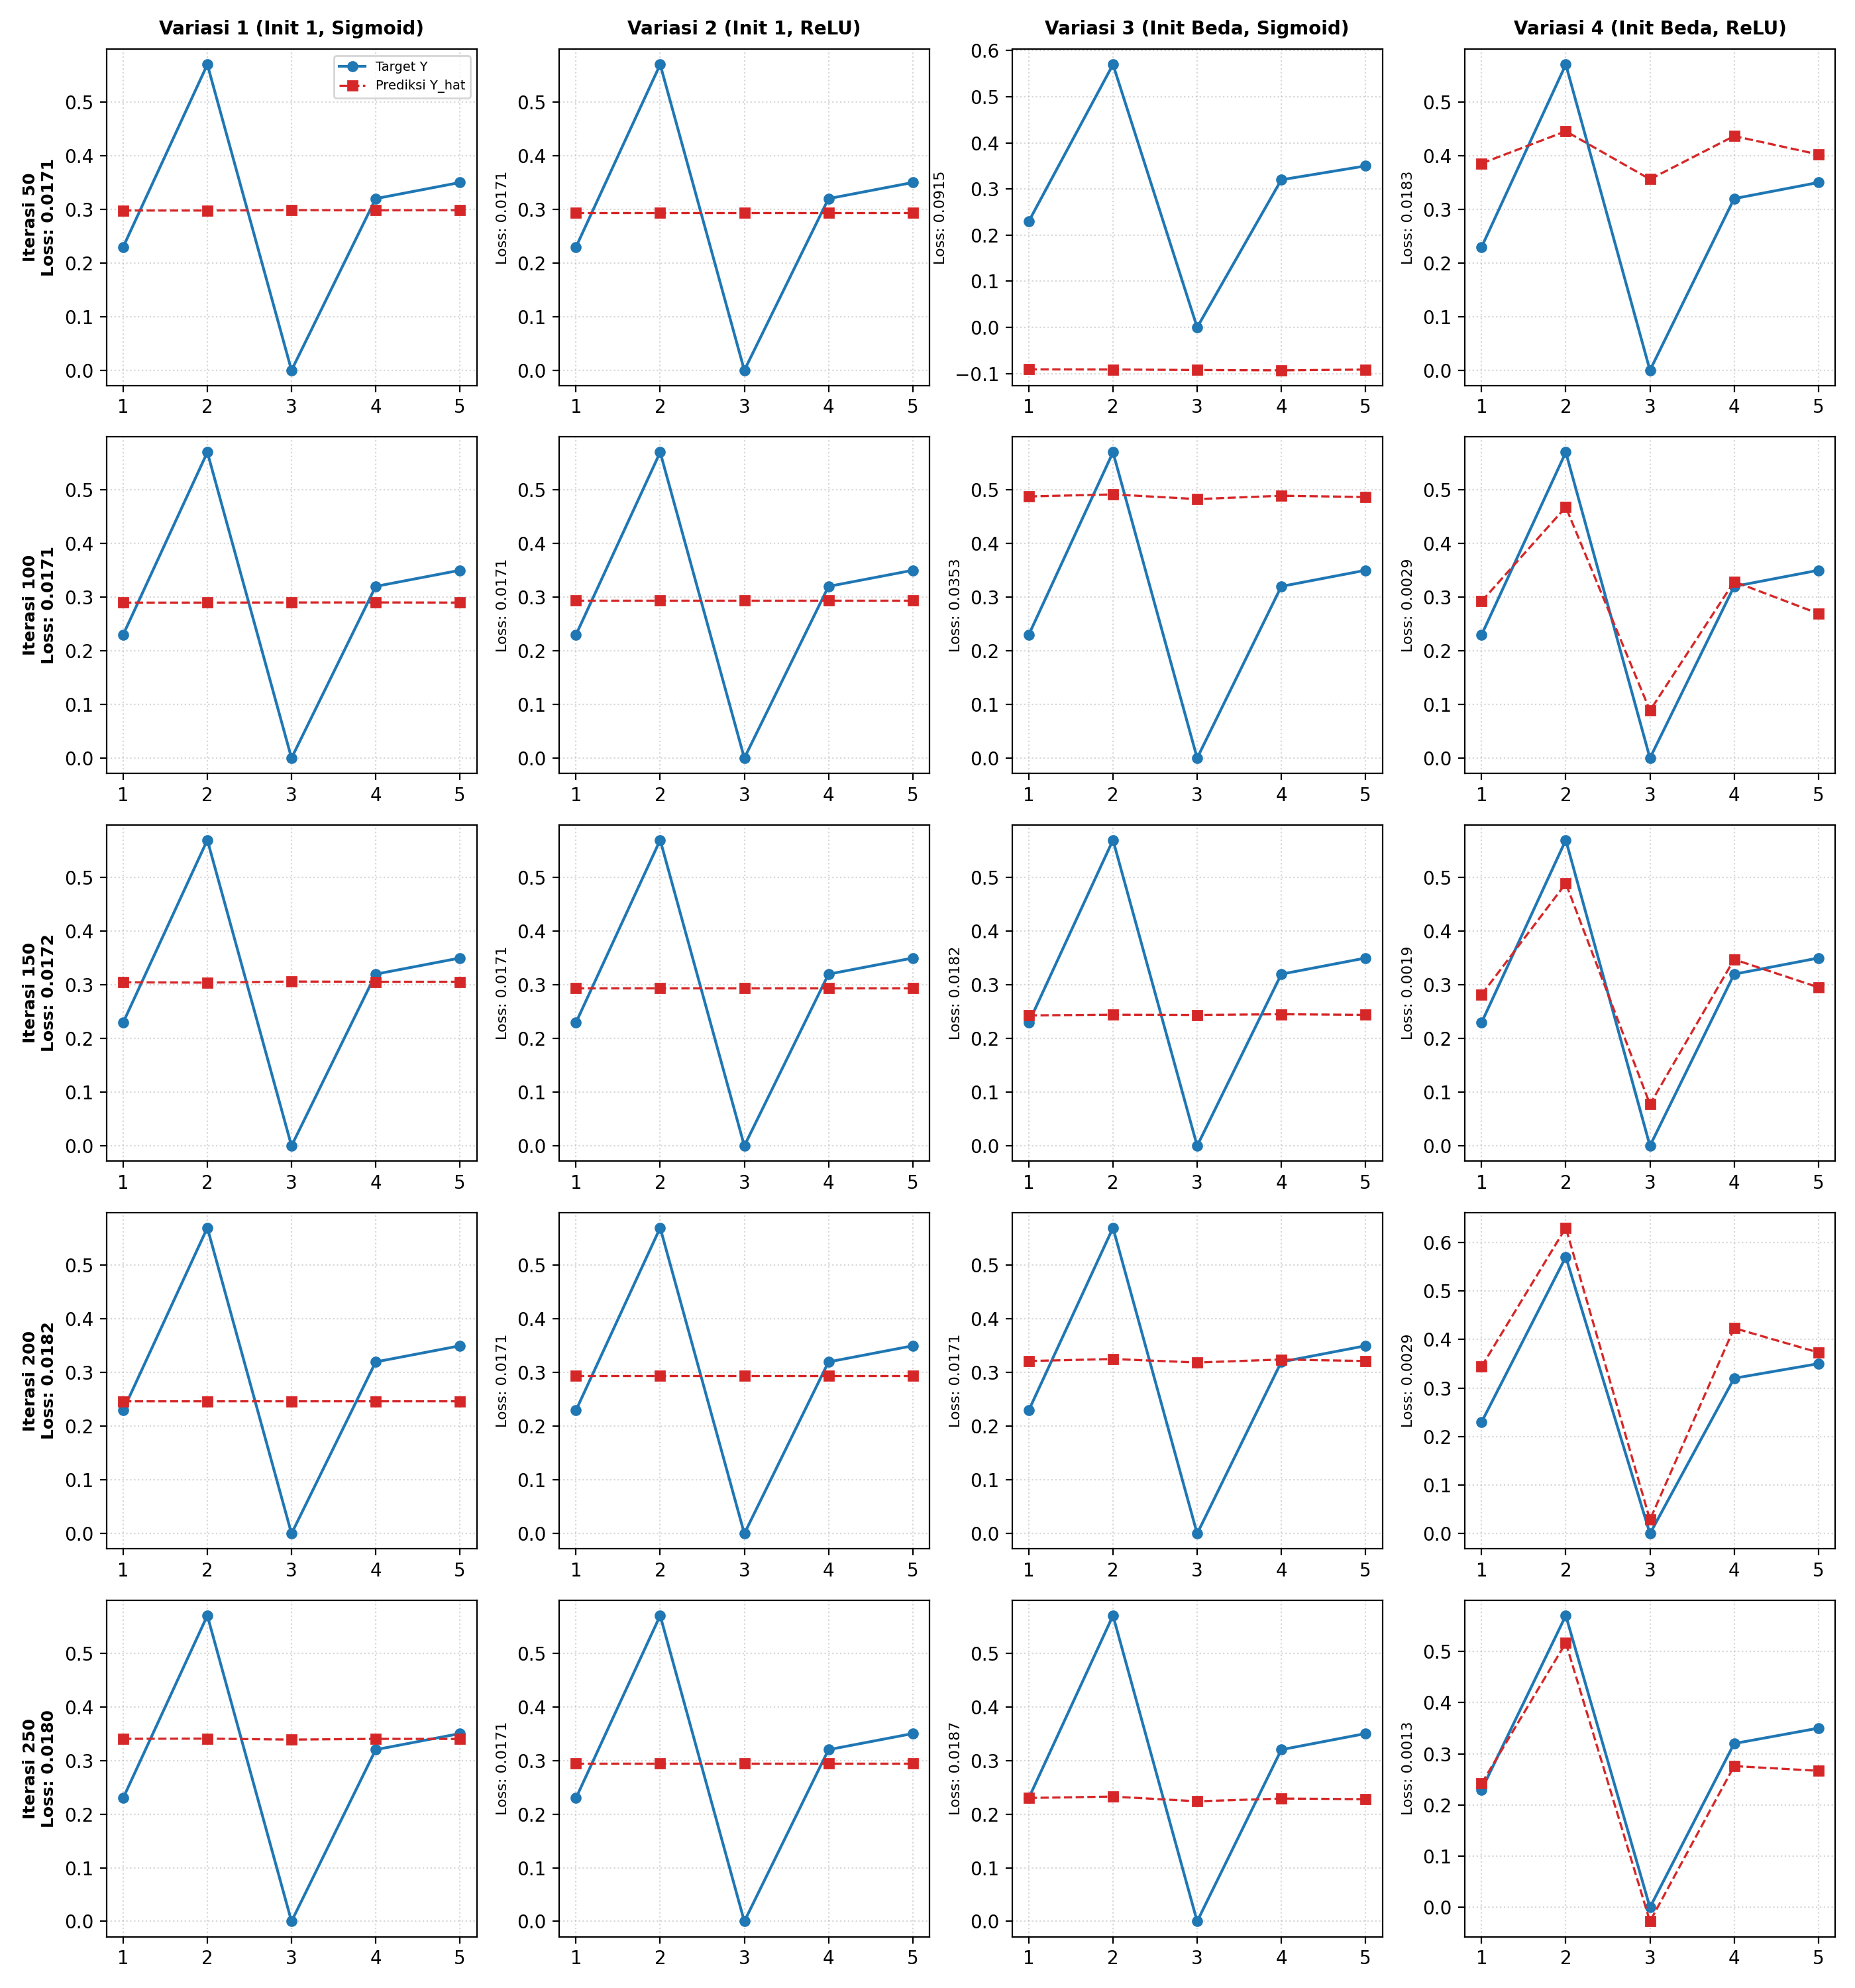
\includegraphics[width=0.98\textwidth]{grid_distribusi_r3_r1_part1.png}
    \caption{Visualisasi Komparasi Target vs Prediksi Bobot Berdistribusi $\mathbb{R}^3 \to \mathbb{R}^1$ (Bagian 1: Iterasi 50 s.d. 250).}
    \label{fig:grid_distribusi_r1_p1}
\end{figure}

\clearpage
\begin{figure}[H]
    \centering
    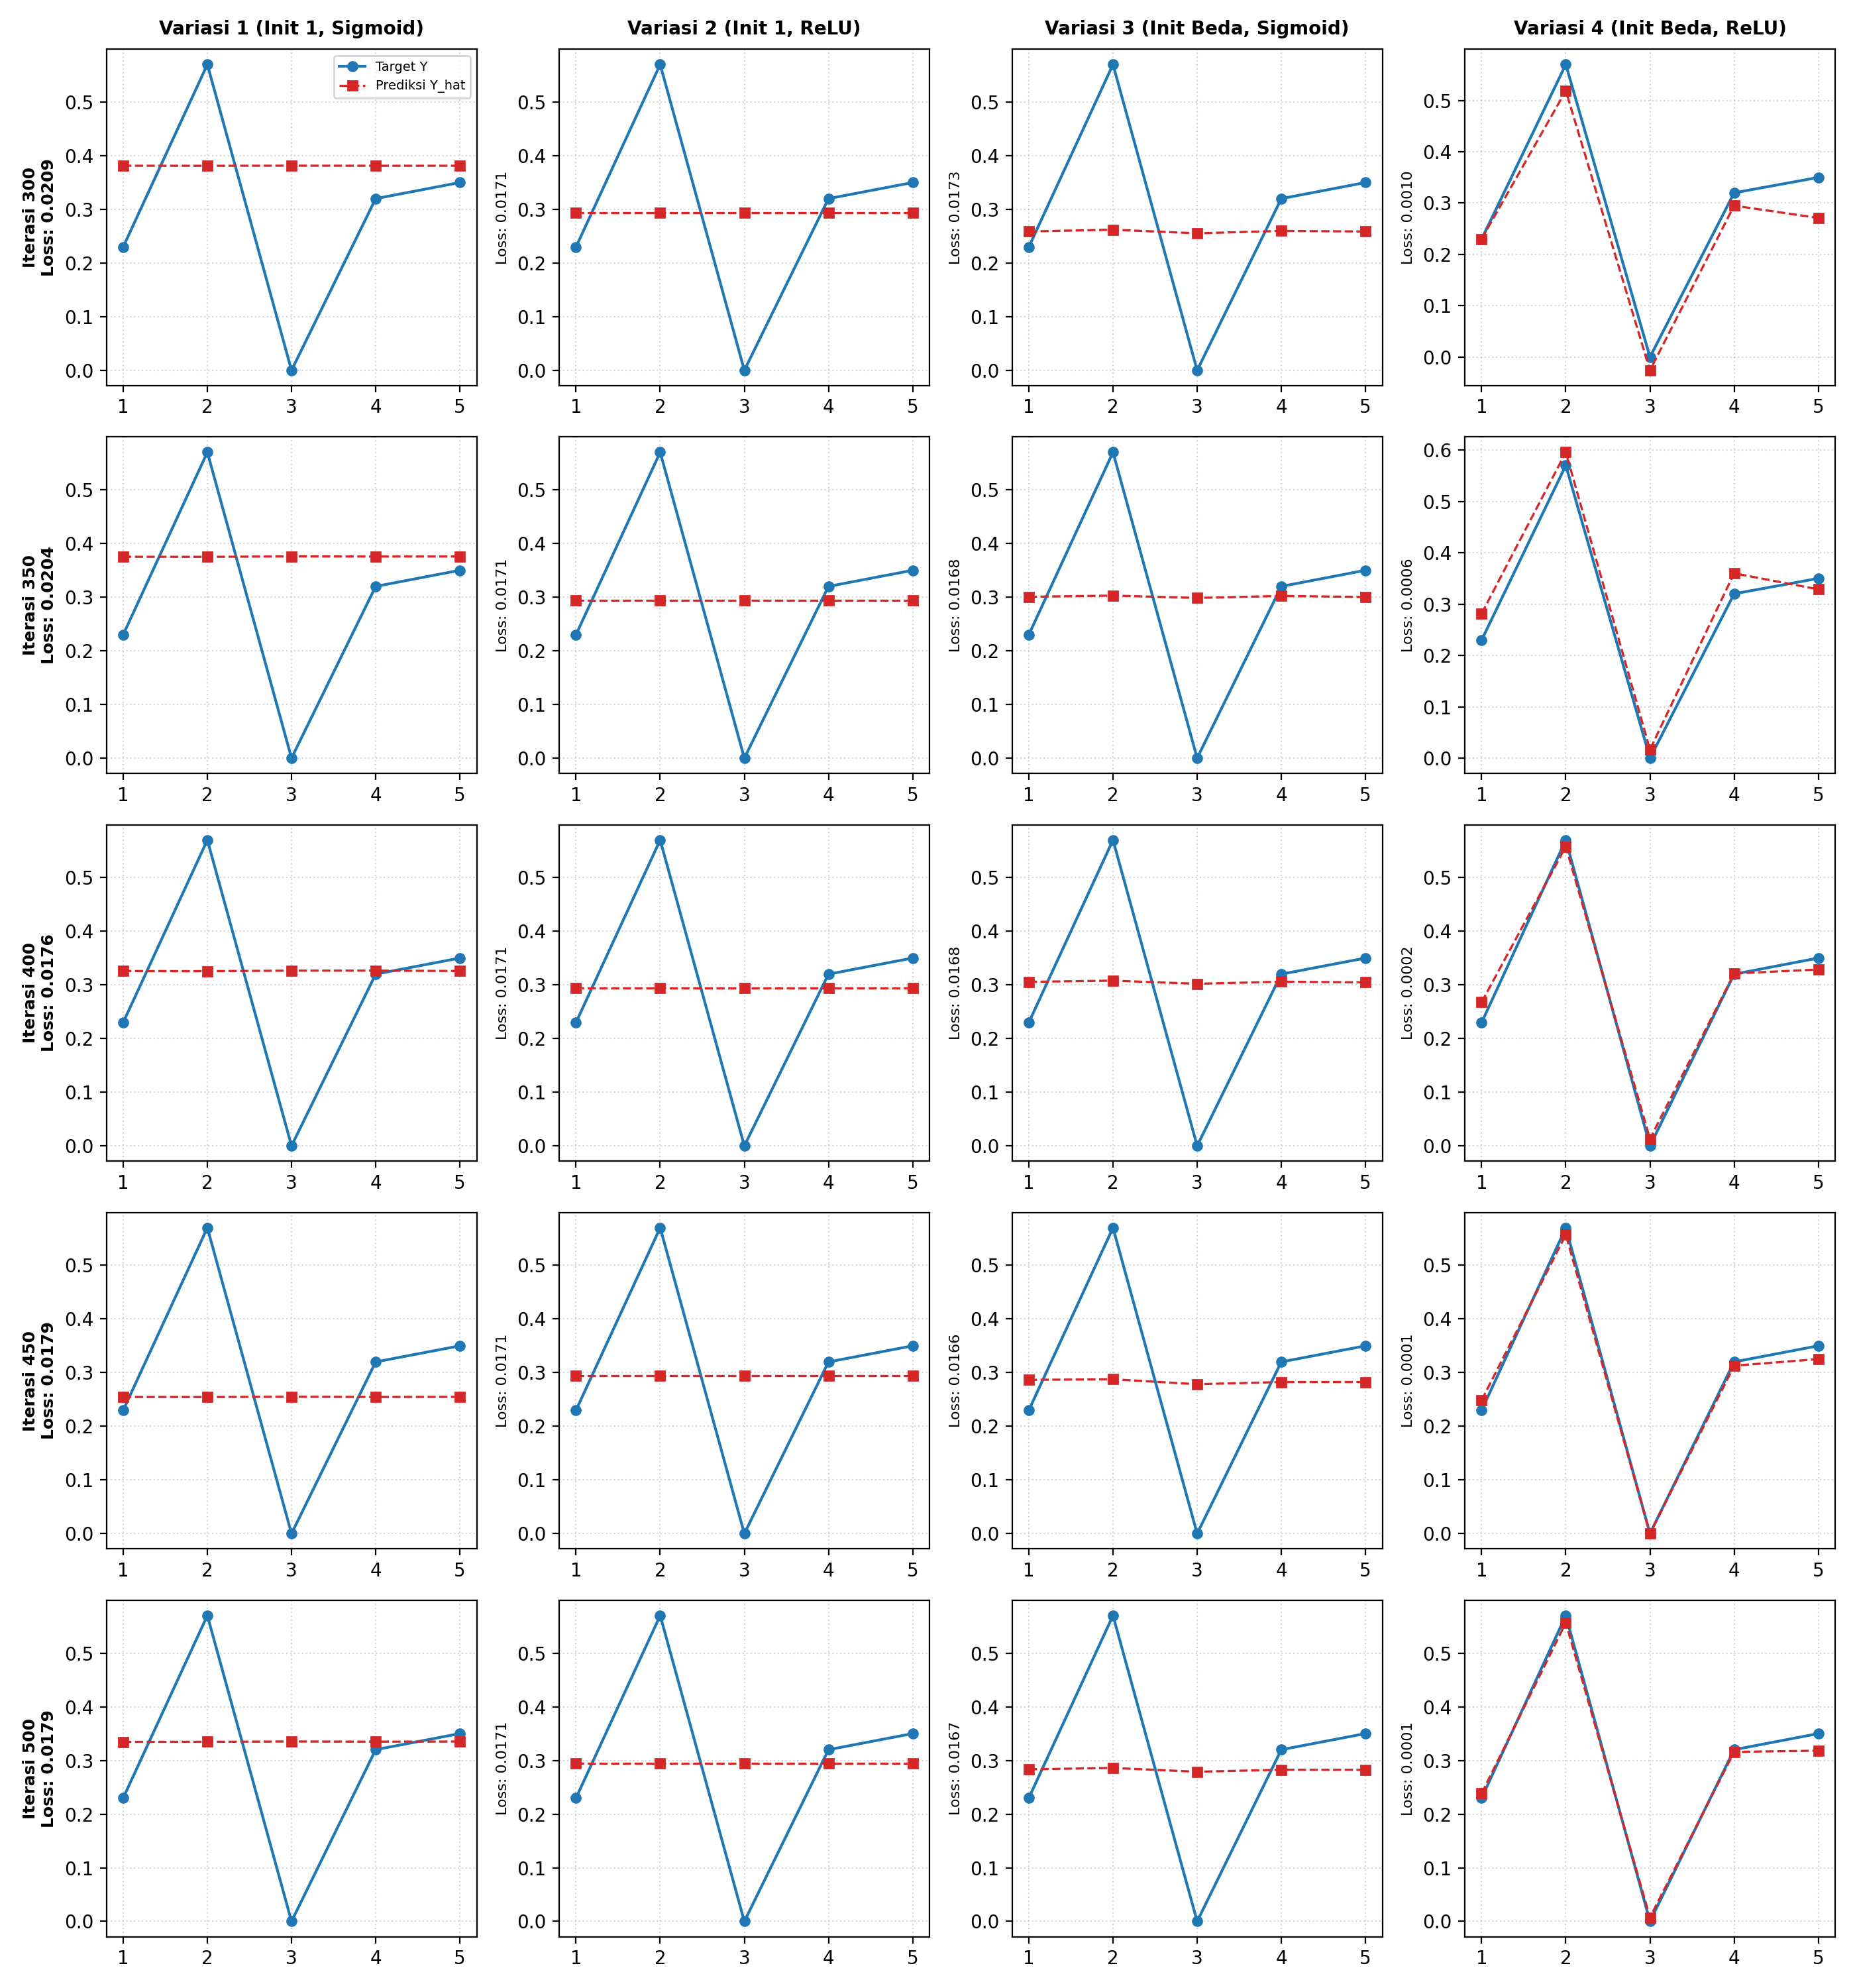
\includegraphics[width=0.98\textwidth]{grid_distribusi_r3_r1_part2.png}
    \caption{Visualisasi Komparasi Target vs Prediksi Bobot Berdistribusi $\mathbb{R}^3 \to \mathbb{R}^1$ (Bagian 2: Iterasi 300 s.d. 500).}
    \label{fig:grid_distribusi_r1_p2}
\end{figure}

\clearpage
\subsubsection{Visualisasi Kurva Fungsi Loss: Bobot Berdistribusi \texorpdfstring{$\mathbb{R}^3 \to \mathbb{R}^1$}{R3 -> R1}}
\label{subsubsec:loss_distribusi_r1}

\begin{figure}[H]
    \centering
    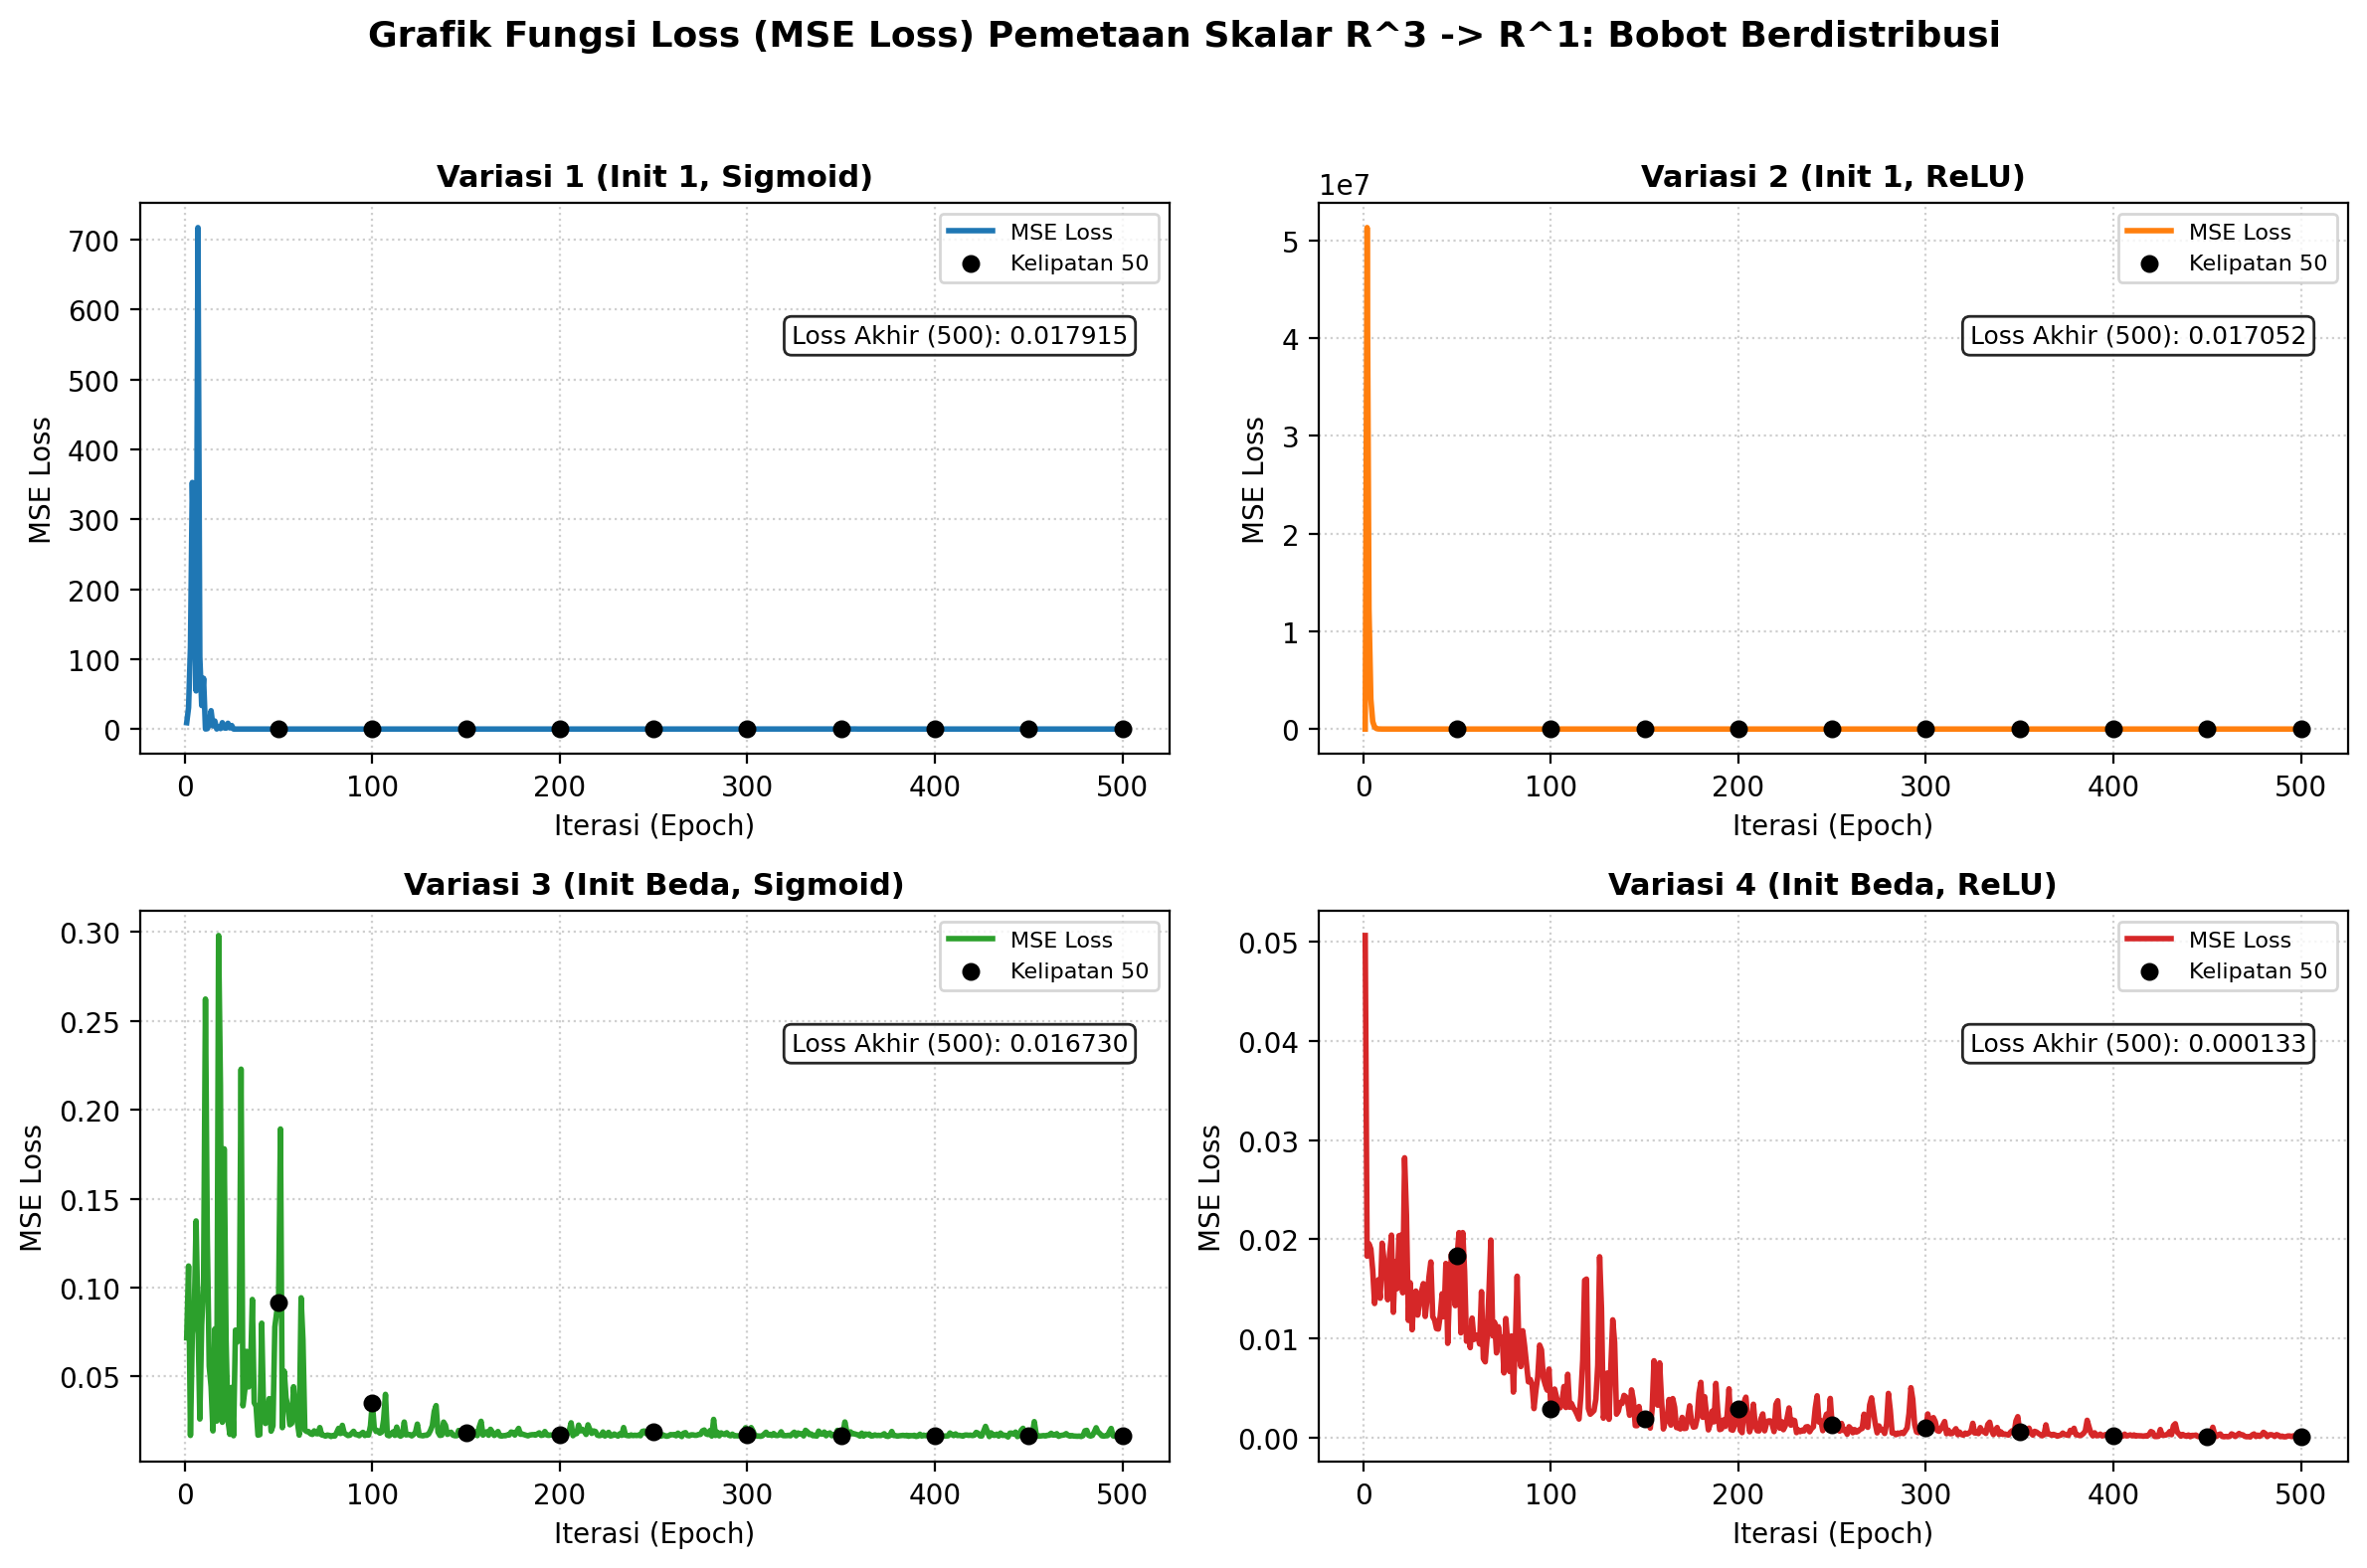
\includegraphics[width=0.98\textwidth]{loss_distribusi_r3_r1.png}
    \caption{Grafik Fungsi Loss (MSE Loss) Pemetaan Skalar $\mathbb{R}^3 \to \mathbb{R}^1$ Bobot Berdistribusi pada 4 Variasi (Iterasi 1 s.d. 500).}
    \label{fig:loss_distribusi_r1}
\end{figure}

% -------------------------------------------------------------------------
\clearpage
\subsection{Subkasus 2: Pemetaan Multi-Output \texorpdfstring{$\mathbb{R}^3 \to \mathbb{R}^2$}{R3 -> R2}}
\label{subsec:distribusi_r3_r2}

\noindent Parameter luaran berdimensi $M^{(3)}, \Sigma^{(3)} \in \mathbb{R}^{6 \times 2}$ dan $\mathbf{b}^{(3)} \in \mathbb{R}^{1 \times 2}$.

\subsubsection{Tabel Komparasi 4 Variasi: Bobot Berdistribusi \texorpdfstring{$\mathbb{R}^3 \to \mathbb{R}^2$}{R3 -> R2}}
\label{subsubsec:tabel_distribusi_r2}

\begin{table}[H]
    \centering
    \small
    \caption{Perbandingan Nilai MSE Loss ($\mathcal{L}$) Setiap Kelipatan 50 Iterasi pada Pemetaan Multi-Output $\mathbb{R}^3 \to \mathbb{R}^2$ (Bobot Berdistribusi).}
    \label{tab:komparasi_distribusi_r2}
    \begin{tabularx}{\textwidth}{c *{4}{>{\centering\arraybackslash}X}}
        \toprule
        \textbf{Iterasi} & \textbf{Variasi 1} & \textbf{Variasi 2} & \textbf{Variasi 3} & \textbf{Variasi 4} \\
        \textbf{($n$)} & \textbf{(Init 1, Sig)} & \textbf{(Init 1, ReLU)} & \textbf{(Init Beda, Sig)} & \textbf{(Init Beda, ReLU)} \\
        \midrule
        1    & 27.238163 & 678.414583 & 0.069550 & 0.071959 \\
        2    & 142.937650 & 5053449.035663 & 0.036804 & 0.029456 \\
        50   & 0.025185 & 0.025144 & 0.034273 & 0.017025 \\
        100  & 0.031335 & 0.025144 & 0.025606 & 0.005747 \\
        150  & 0.025144 & 0.025144 & 0.025696 & 0.002645 \\
        200  & 0.025199 & 0.025144 & 0.024771 & 0.002379 \\
        250  & 0.025144 & 0.025144 & 0.025313 & 0.002095 \\
        300  & 0.025144 & 0.025144 & 0.025239 & 0.002183 \\
        350  & 0.025301 & 0.025144 & 0.025527 & 0.001722 \\
        400  & 0.025585 & 0.025144 & 0.025169 & 0.001491 \\
        450  & 0.025173 & 0.025144 & 0.024588 & 0.001571 \\
        500  & 0.025144 & 0.025144 & 0.024709 & 0.001322 \\
        \bottomrule
    \end{tabularx}
\end{table}

\subsubsection{Visualisasi Kurva Fungsi Loss: Bobot Berdistribusi \texorpdfstring{$\mathbb{R}^3 \to \mathbb{R}^2$}{R3 -> R2}}
\label{subsubsec:loss_distribusi_r2}

\begin{figure}[H]
    \centering
    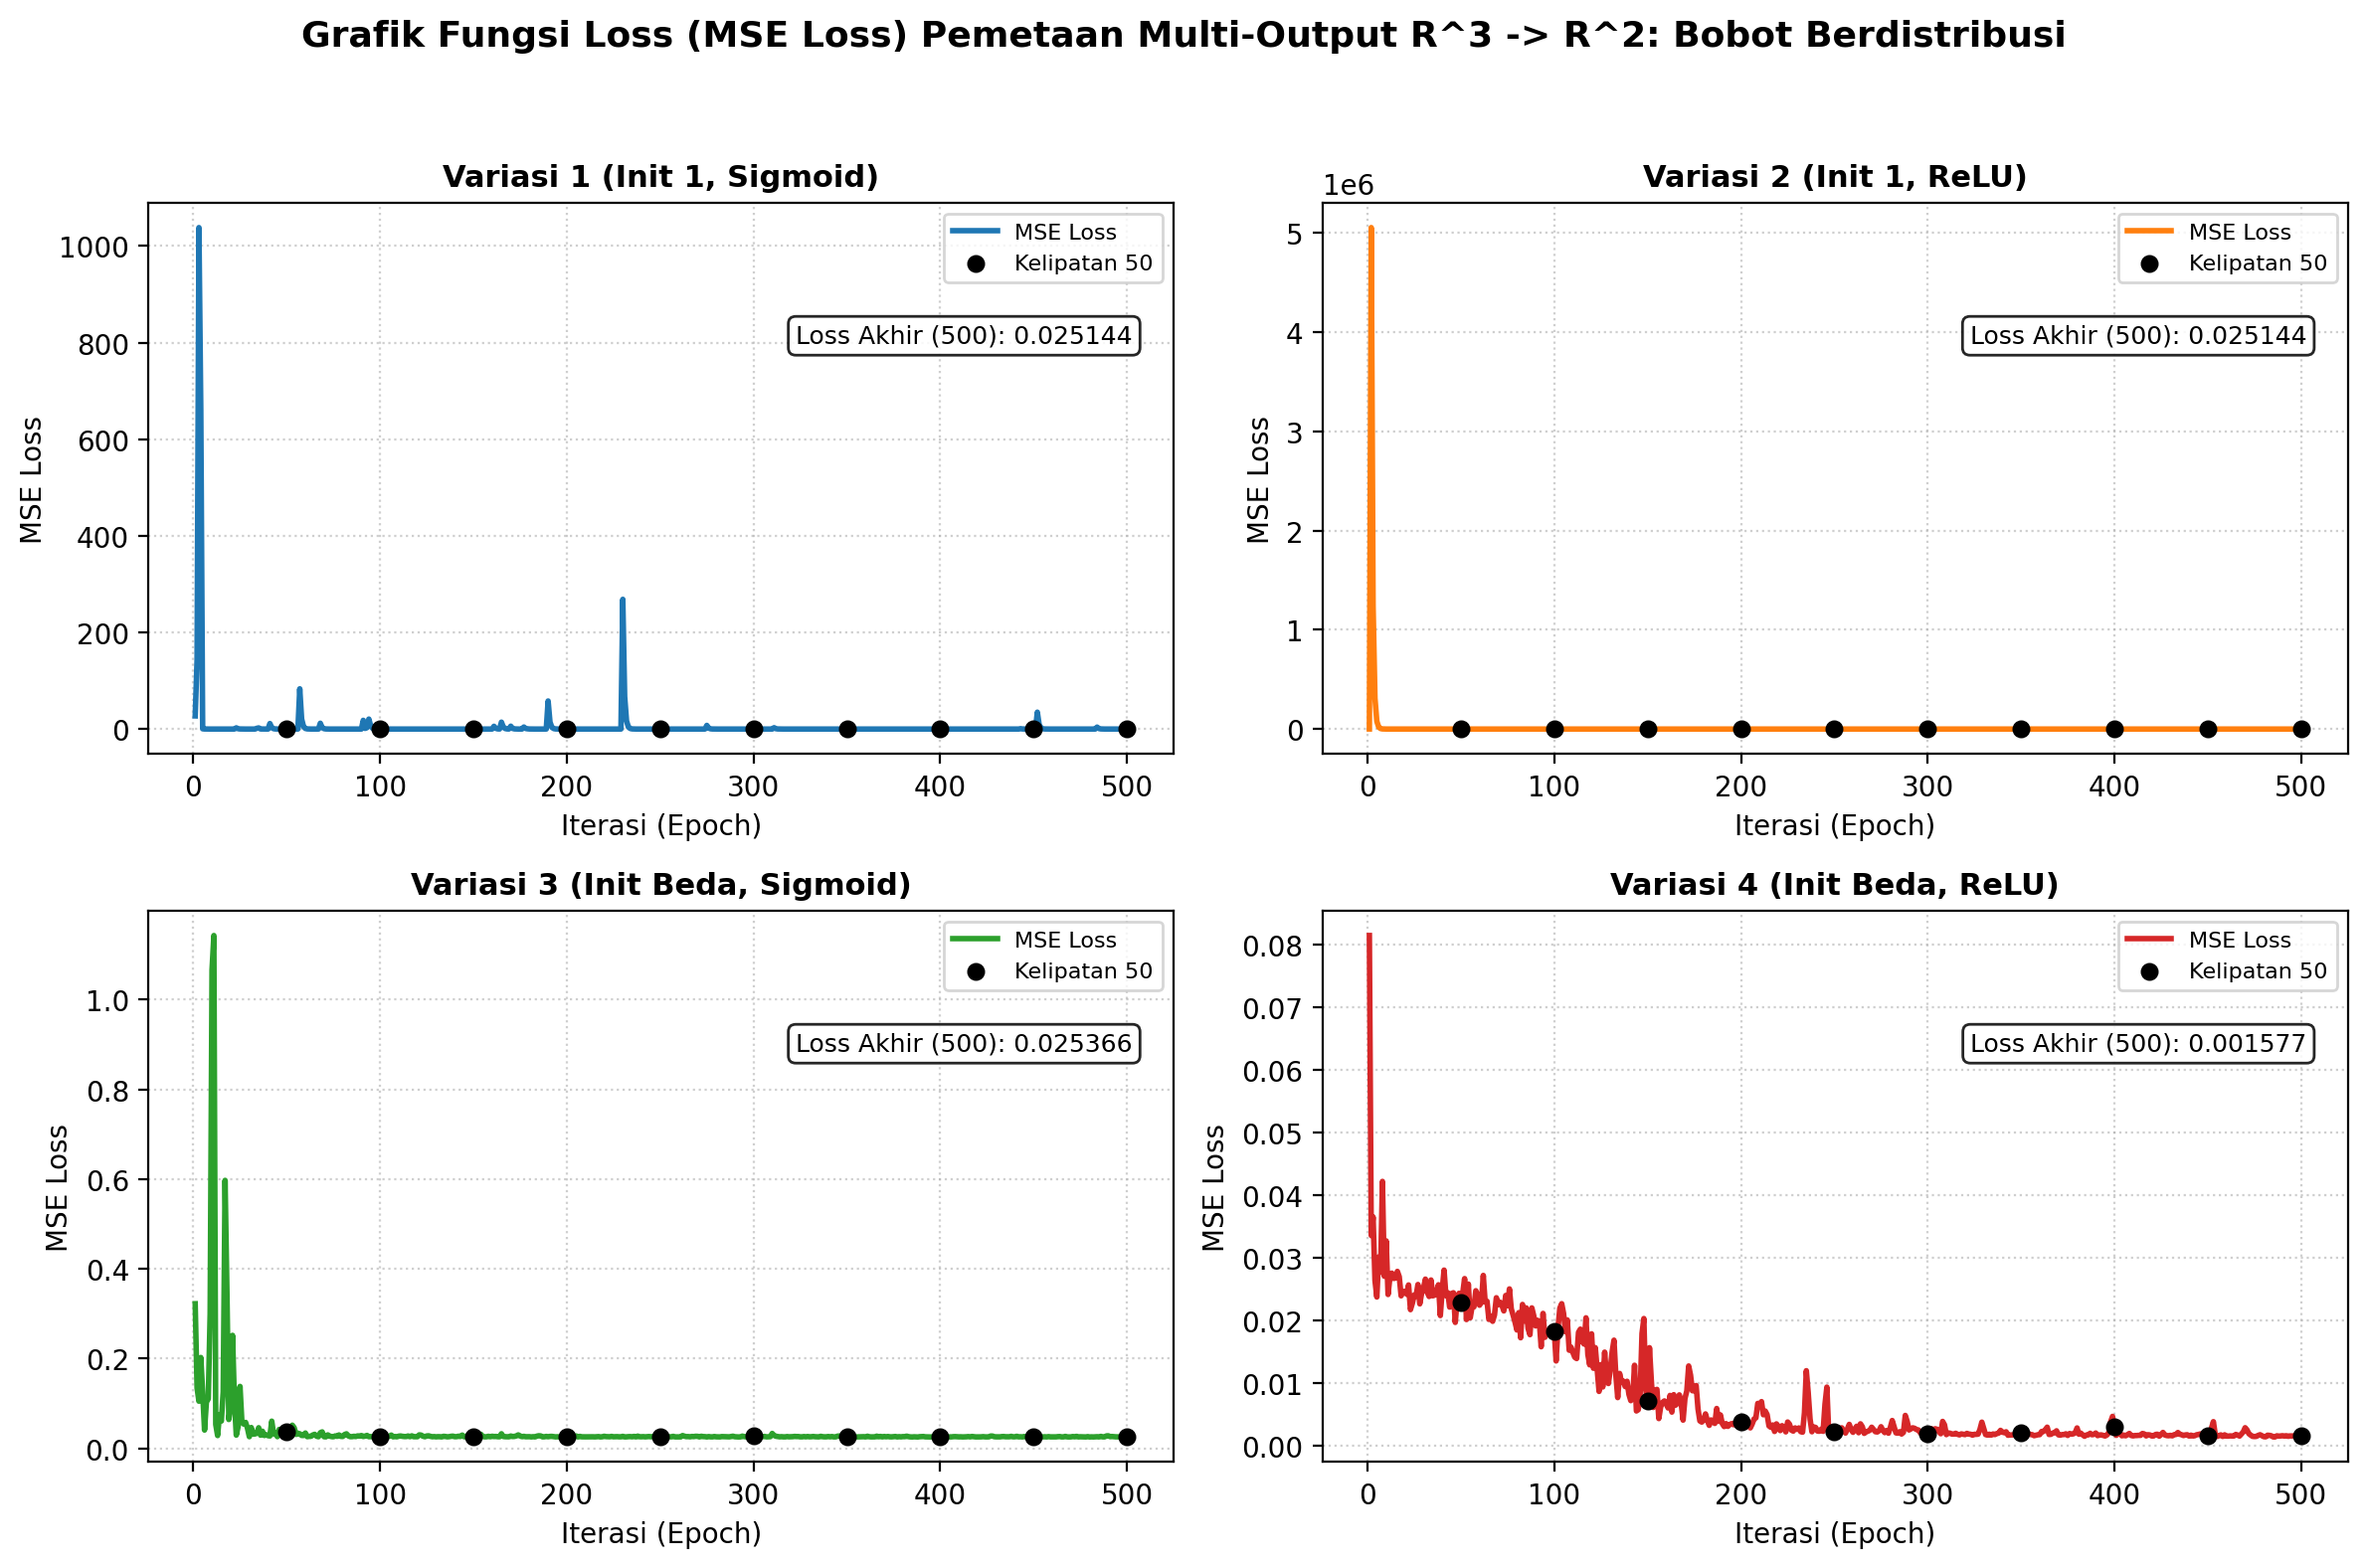
\includegraphics[width=0.98\textwidth]{loss_distribusi_r3_r2.png}
    \caption{Grafik Fungsi Loss (MSE Loss) Pemetaan Multi-Output $\mathbb{R}^3 \to \mathbb{R}^2$ Bobot Berdistribusi pada 4 Variasi (Iterasi 1 s.d. 500).}
    \label{fig:loss_distribusi_r2}
\end{figure}

\end{document}
